% Chapter 1: Introduction
% Contains:
%   An introduction to random graph theory
%   Basic results on the size of random graph components
%   Basic results on the critical window
%   The main theorem:
%      Motivation
%      The Brownian motion
%      Complete statement
%   Overview of coming proof

\chapter{Introduction}
\fxnote{Update title.}

A brief introduction.
\lipsum[100]

\section{The Erdös-Renyi random graph}
%%%%%%%%%%%%%%%%%%%%%%%%%%%%%%%%%%%%%%%%%%%%%%%%%%%%%%%%%%%%
% SECTION: The Erdös-Renyi random graph
%%%%%%%%%%%%%%%%%%%%%%%%%%%%%%%%%%%%%%%%%%%%%%%%%%%%%%%%%%%%

In their paper, Erdös and Renyi proposed a model of random graph that is now known as the Erdös-Renyi random graph.
There are several ways to construct this random graph which we will briefly introduce,
starting with the historic models used in this first paper 
and continuing with the equivalent model which provides the basis for Aldous' paper and consequently this thesis.

We denote by $G_{n,M}$ the set of graphs on $n$ vertices with $M$ edges that are
\begin{enumerate}
	\item undirected,
	\item without slings, i.e. there is no edge $(v,v)$ for some vertex $v$,
	\item without parallel edges, i.e. there can be at most one edge $(v_1, v_2)$ for each pair of vertices.
\end{enumerate}
A graph in $G_{n,M}$ can be constructed by choosing $M$ out of the $\binom{n}{2}$ possible edges between the vertices,
which leads to a total number of graphs
\begin{equation}
	|G_{n,M}| = \binom{\binom{n}{2}}{M}.
\end{equation}
The Erdös-Renyi random graph $\Gcal(n, M)$ is now obtained by choosing one element of $G_{n,M}$ at random
with equal probability for each graph, where the number of edges is usually dependent on the number of vertices, $M = M(n)$.

An equivalent definition provides the following process:
Starting with a graph on $n$ vertices with $0$ edges at time $t=1$, 
pick one of the $\binom{n}{2}$ possible edges at random with equal probability for each edge,
label it $e_1$.
At time $t=2$ pick one of the remaining $\binom{n}{2}-1$ edges, again all remaining edges being equiprobable,
and denote it by $e_2$.
Continue until $M$ edges have been chosen at time $t=M$.
The graph on vertices $\{1, \dots, n\}$ with edges $\{e_1, \dots, e_M\}$ is the desired Erdös-Renyi random graph.

Using these definitions Erdös and Renyi prove that,
when increasing the number of edges $M(n)$,
the sizes of connected components undergo distinct phases leading from small sparse components and unconnected vertices
to one giant component and eventually a completely connected graph.

Most current literature and the paper we are studying uses a slightly different approach to constructing the Erdös-Renyi random graph.
Given a set of vertices $\{1, \dots, n\}$ and an edge-probability $\p = p(n)$
we take every edge $(v_1, v_2)$ and add it to the set of edges of the random graph with probability $\p$ independently.
We denote a random object constructed this way by $\Gcal(n, \p)$ and expect a realisation of the random graph to have $\binom{n}{2}\p$ edges.
When increasing the probability $\p$ from $0$ to $1$ the resulting random graph undergoes the same so-called phase transitions
discovered by Erdös and Renyi.

While the results of the original paper hold for small and large $M(n)$,
the critical phase transistion happening around $M(n) = \frac{n}{2}$ or $\p = \frac{1}{n}$
was later discovered to be imprecise.
\fxnote{Add reference from hofstad somewhere.}
The following section will provide a more precise introduction to the different phases a random graph undergoes
with increasing number of edges.


\section{General results on component sizes}
%%%%%%%%%%%%%%%%%%%%%%%%%%%%%%%%%%%%%%%%%%%%%%%%%%%%%%%%%%%%
% SECTION: General results on component sizes
%%%%%%%%%%%%%%%%%%%%%%%%%%%%%%%%%%%%%%%%%%%%%%%%%%%%%%%%%%%%

In this section we discuss previous results on component sizes in the Erdös-Renyi random graph.
We begin with the subcritical graph, that is
$\Gcal(n, \p)$ with $\p < \frac{1}{n}$.

Define $\lambda = \p n$ and $I_{\lambda}$ as the large deviation rate functions for Poisson random variables with mean $\lambda$,
that is
\begin{equation}
	I_{\lambda} = \lambda - 1 - \log(\lambda).
\end{equation}

The following theorem provides an upper bound on the size of $\Ccal_{\max}$, the largest component of $\Gcal$.
\begin{theorem}[Lower bound on largest subcritical component, {\cite[Theorem 4.4, p.125]{vanderHofstad.2016}}]
	Fix $\lambda < 1$. 
	Then, for all $a > 1/I_{\lambda}$, 
	there exists $\delta = \delta(a, \lambda)$ such that
	\begin{equation}
		\Prob( |\Ccal_{\max}| \geq a \log n ) = \BigO{n^{-\delta}}.
	\end{equation}
\end{theorem}

The next theorem gives an upper bound for the size of $\Ccal_{\max}$.
\begin{theorem}[Upper bound on largest subcritical component, {\cite[Theorem 4.5, p.125]{vanderHofstad.2016}}]
	Fix $\lambda < 1$. 
	Then, for all $a < 1/I_{\lambda}$, 
	there exists $\delta = \delta(a, \lambda)$ such that
	\begin{equation}
	\Prob( |\Ccal_{\max}| \leq a \log n ) = \BigO{n^{-\delta}}.
	\end{equation}
\end{theorem}

Together, these theorems imply
\begin{equation}
	\frac{|\Ccal_{\max}|}{\log n} \rightarrow_p 1/I_{\lambda}.
\end{equation}

We have established that, for $\p n < 1$, the expected largest component size will be of order $\log n$.

Consider the opposite case, $\lambda = \p n > 1$. 
Denote by $\xi_\lambda = 1 - \eta_n\lambda$ the survival probability of a Poisson branching process with mean offspring $\lambda$.
Note that $\xi_\lambda > 0$ since $\lambda > 1$.
Any vertex is part of a large component with probability $\xi_\lambda$, 
therefore we will expect around $n \xi_\lambda$ vertices being part of large connected components.
The following theorem now states that all of these vertices are, in fact, part of the same connected component, which we call the giant component.
\fxnote{Add explanation for Poisson branching process}
\begin{theorem}[Law of large numbers for giant component, {\cite[Theorem 4.8, p.131]{vanderHofstad.2016}}]
	Fix $\lambda>1$.
	Then, for all $\nu \in (\frac{1}{2}, 1)$, there exists $\delta = \delta(\nu, \lambda)$ such that
	\begin{equation}
		\Prob\left( \left| |\Ccal_{\max}| - n \xi_\lambda \right| \geq n^{\nu}\right) = \BigO{n^{-\delta}}.
	\end{equation}
\end{theorem}

\fxnote{What size is this giant component?}

To recap: For $n \p < 1$ we expect many small clusters of size at most $\log n$,
for $n \p > 1$ we expect one giant component, rapidly approaching size $n$.
But what happens around $n \p \approx 1$?
As it turns out, the emergence of the giant component occurs quite rapidly,
such that shortly after $n \p = 1$ most graphs do not have any component of order between $\frac{1}{2}\n{2}{3}$ and $\n{2}{3}$.

The following theorem provides an approximation of the time of emergence of the giant component,
seeing the random graph on $n$ vertices as a graph process,
starting at $t=0$ with $0$ edges, adding one random edge at every time step.
We would therefore expect the emergence starting around time $\binom{2}{n}\frac{1}{n} \approx \frac{1}{2}n$. 

\begin{theorem}[Emergence of the giant component, {\cite[Theorem 6.8, p.142]{Bollobas.2001}}]
	Almost every graph process $\Gcal = (\Gcal_t)_0^n$ is such that 
	for every $t \geq t_1 = \floor{ n/2 + 2(\log n)^{1/2}\n{2}{3} }$ 
	the graph $\Gcal_t$ has a unique component of order at least $\n{2}{3}$ and the other components have at most $\frac{1}{2}\n{2}{3}$
\end{theorem}

As it turns out, there is a so-called critical window in which the component sizes are not of size $\log n$ and there is no giant component yet.
We call a random graph $\Gcal(n, n^{-1} + t\n{-4}{3})$ critical for $t \in \Real$.
The next theorem provides a approximation of the size of the largest component in a critical random graph.

\begin{theorem}[Largest critical cluster, {\cite[Theorem 5.1, p.150]{vanderHofstad.2016}}] \label{T: largest critical cluster}
	Let $\lambda = 1 + \pp\n{-1}{3}$, with $\pp \in \Real$.
	There exists a constant $b = b(\pp)$ such that for all $\omega > 1$,
	\begin{equation}
		\Prob\left( \omega^{-1} \n{2}{3} \leq |\Ccal_{\max}| \leq \omega \n{2}{3}\right) \geq 1 - \frac{b}{\omega}.
	\end{equation}	
\end{theorem}

Therefore, rescaling the size of the largest component by $\n{-2}{3}$,
it is contained in an interval $[\omega^{-1}, \omega]$ with hight probability.

But is it possible to provide a similar statement not only for the largest, but for all components in a critical random graph?
Aldous notes that previous to his paper
the convergence of the rescaled component sizes to some limit process was generally assumed to be true,
although never explicitly proven.
He therefore provides the following \emph{folk theorem},
which will be proven in more precise form in the course of this thesis.

\begin{folktheorem} \label{T: folk theorem}
	Let $\Cnt(1) \geq \Cnt(2) \geq \dots$ be the ordered component sizes of
	$\Gcal(n, n^{-1} + \pp\n{-4}{3})$ and let $\sigmant(j)$ be the surplus of the corresponding component.
	Then
	\begin{equation}
		( \n{-2}{3} ( \Cnt(j), \sigmant(j) ), \; j \geq 1 ) 
		\rightarrow_d
		( (\Ct(j), \sigmat), \; j \geq 1 )
		= ( \Ctbold, \sigmatbold ),
	\end{equation}
	as $n \rightarrow \infty$ for some limit $( \Ctbold, \sigmatbold )$
	with $0 < \Ct(j) < \infty$ and $0 \leq \sigmatbold(j) < \infty$ almost surely for each $j \geq 1$.
\end{folktheorem}



\section{Main statements of this thesis}
%%%%%%%%%%%%%%%%%%%%%%%%%%%%%%%%%%%%%%%%%%%%%%%%%%%%%%%%%%%%
% SECTION: Main statements of this thesis
%%%%%%%%%%%%%%%%%%%%%%%%%%%%%%%%%%%%%%%%%%%%%%%%%%%%%%%%%%%%

In this section we state the main results of this thesis,
which is a refinement of Theorem~\ref{T: largest critical cluster}.
While previously the size of largest component was only estimated to be of order $\n{2}{3}$,
the following theorem will give a limit distribution for all component sizes, downscaled by $\n{-2}{3}$.

Denote by $W$ the standard Brownian motion. 
For a fixed parameter $\pp \in \Real$ we call the process $\Wt$, defined by
\begin{equation}
	\Wt(s) := W(s) + \int_{0}^{s}(t-s)ds = W(s) + ts - \frac{1}{2}s^2,
\end{equation}
the Brownian motion with drift $t-s$ at time $s$.
The central object of our analysis will be the process $\Wt$ and its excursions above past minima.
We reflect $\Wt$ at $0$, defining the process $\Bt$ by
\begin{equation}
	\Bt(s) := \Wt(s) - \min_{u \leq s}\Wt(u)
\end{equation}
and calling it the reflected Brownian motion with drift.

\begin{figure}%
	\centering
	\subfloat[$W(s)$]{% Created by tikzDevice version 0.10.1 on 2017-01-16 15:57:32
% !TEX encoding = UTF-8 Unicode
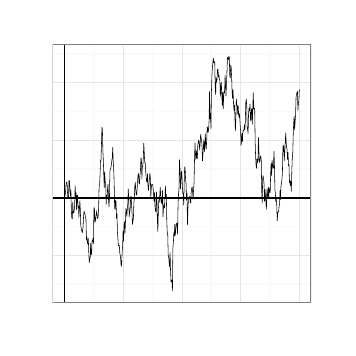
\begin{tikzpicture}[x=1pt,y=1pt]
\definecolor{fillColor}{RGB}{255,255,255}
\path[use as bounding box,fill=fillColor,fill opacity=0.00] (0,0) rectangle (108.41,108.41);
\begin{scope}
\path[clip] (  0.00,  0.00) rectangle (108.40,108.41);
\definecolor{drawColor}{RGB}{255,255,255}
\definecolor{fillColor}{RGB}{255,255,255}

\path[draw=drawColor,line width= 0.6pt,line join=round,line cap=round,fill=fillColor] (  0.00,  0.00) rectangle (108.41,108.41);
\end{scope}
\begin{scope}
\path[clip] (  9.00,  9.00) rectangle (102.41,102.41);
\definecolor{fillColor}{RGB}{255,255,255}

\path[fill=fillColor] (  9.00,  9.00) rectangle (102.40,102.41);
\definecolor{drawColor}{gray}{0.98}

\path[draw=drawColor,line width= 0.6pt,line join=round] (  9.00, 15.75) --
	(102.41, 15.75);

\path[draw=drawColor,line width= 0.6pt,line join=round] (  9.00, 36.56) --
	(102.41, 36.56);

\path[draw=drawColor,line width= 0.6pt,line join=round] (  9.00, 57.36) --
	(102.41, 57.36);

\path[draw=drawColor,line width= 0.6pt,line join=round] (  9.00, 78.17) --
	(102.41, 78.17);

\path[draw=drawColor,line width= 0.6pt,line join=round] (  9.00, 98.98) --
	(102.41, 98.98);

\path[draw=drawColor,line width= 0.6pt,line join=round] ( 23.86,  9.00) --
	( 23.86,102.41);

\path[draw=drawColor,line width= 0.6pt,line join=round] ( 45.09,  9.00) --
	( 45.09,102.41);

\path[draw=drawColor,line width= 0.6pt,line join=round] ( 66.32,  9.00) --
	( 66.32,102.41);

\path[draw=drawColor,line width= 0.6pt,line join=round] ( 87.55,  9.00) --
	( 87.55,102.41);
\definecolor{drawColor}{gray}{0.90}

\path[draw=drawColor,line width= 0.2pt,line join=round] (  9.00, 26.15) --
	(102.41, 26.15);

\path[draw=drawColor,line width= 0.2pt,line join=round] (  9.00, 46.96) --
	(102.41, 46.96);

\path[draw=drawColor,line width= 0.2pt,line join=round] (  9.00, 67.77) --
	(102.41, 67.77);

\path[draw=drawColor,line width= 0.2pt,line join=round] (  9.00, 88.58) --
	(102.41, 88.58);

\path[draw=drawColor,line width= 0.2pt,line join=round] ( 13.25,  9.00) --
	( 13.25,102.41);

\path[draw=drawColor,line width= 0.2pt,line join=round] ( 34.47,  9.00) --
	( 34.47,102.41);

\path[draw=drawColor,line width= 0.2pt,line join=round] ( 55.70,  9.00) --
	( 55.70,102.41);

\path[draw=drawColor,line width= 0.2pt,line join=round] ( 76.93,  9.00) --
	( 76.93,102.41);

\path[draw=drawColor,line width= 0.2pt,line join=round] ( 98.16,  9.00) --
	( 98.16,102.41);
\definecolor{drawColor}{RGB}{0,0,0}

\path[draw=drawColor,line width= 0.2pt,line join=round] ( 13.25, 46.96) --
	( 13.42, 47.31) --
	( 13.59, 48.26) --
	( 13.76, 50.06) --
	( 13.92, 52.38) --
	( 14.09, 52.63) --
	( 14.26, 52.15) --
	( 14.43, 47.90) --
	( 14.60, 46.67) --
	( 14.77, 47.37) --
	( 14.94, 53.27) --
	( 15.11, 52.86) --
	( 15.28, 49.46) --
	( 15.45, 47.50) --
	( 15.62, 49.90) --
	( 15.79, 42.11) --
	( 15.96, 39.48) --
	( 16.13, 39.30) --
	( 16.30, 45.30) --
	( 16.47, 41.47) --
	( 16.64, 41.40) --
	( 16.81, 42.32) --
	( 16.98, 44.40) --
	( 17.15, 51.35) --
	( 17.32, 47.17) --
	( 17.49, 48.81) --
	( 17.66, 42.58) --
	( 17.83, 47.74) --
	( 18.00, 47.90) --
	( 18.17, 43.57) --
	( 18.34, 44.21) --
	( 18.51, 39.85) --
	( 18.68, 42.76) --
	( 18.85, 45.92) --
	( 19.02, 42.68) --
	( 19.19, 37.22) --
	( 19.36, 35.67) --
	( 19.53, 35.32) --
	( 19.70, 34.24) --
	( 19.87, 35.15) --
	( 20.04, 36.69) --
	( 20.21, 40.45) --
	( 20.38, 42.10) --
	( 20.55, 41.49) --
	( 20.72, 41.07) --
	( 20.89, 39.70) --
	( 21.06, 39.44) --
	( 21.23, 31.68) --
	( 21.40, 32.83) --
	( 21.57, 30.73) --
	( 21.74, 30.19) --
	( 21.91, 32.22) --
	( 22.08, 27.18) --
	( 22.25, 23.56) --
	( 22.42, 25.01) --
	( 22.59, 25.03) --
	( 22.76, 30.48) --
	( 22.93, 26.53) --
	( 23.10, 26.48) --
	( 23.27, 31.47) --
	( 23.44, 31.08) --
	( 23.61, 32.39) --
	( 23.77, 30.36) --
	( 23.94, 43.21) --
	( 24.11, 43.35) --
	( 24.28, 38.20) --
	( 24.45, 38.32) --
	( 24.62, 40.27) --
	( 24.79, 40.96) --
	( 24.96, 42.25) --
	( 25.13, 39.45) --
	( 25.30, 39.64) --
	( 25.47, 40.03) --
	( 25.64, 43.52) --
	( 25.81, 51.10) --
	( 25.98, 51.35) --
	( 26.15, 55.02) --
	( 26.32, 60.39) --
	( 26.49, 60.42) --
	( 26.66, 66.12) --
	( 26.83, 72.49) --
	( 27.00, 71.69) --
	( 27.17, 63.83) --
	( 27.34, 60.53) --
	( 27.51, 54.88) --
	( 27.68, 50.63) --
	( 27.85, 56.35) --
	( 28.02, 52.47) --
	( 28.19, 52.38) --
	( 28.36, 44.44) --
	( 28.53, 47.88) --
	( 28.70, 46.49) --
	( 28.87, 50.40) --
	( 29.04, 51.87) --
	( 29.21, 46.24) --
	( 29.38, 43.72) --
	( 29.55, 46.89) --
	( 29.72, 56.48) --
	( 29.89, 57.34) --
	( 30.06, 57.75) --
	( 30.23, 58.85) --
	( 30.40, 60.43) --
	( 30.57, 61.35) --
	( 30.74, 65.14) --
	( 30.91, 60.18) --
	( 31.08, 57.39) --
	( 31.25, 52.48) --
	( 31.42, 43.20) --
	( 31.59, 42.79) --
	( 31.76, 46.02) --
	( 31.93, 45.68) --
	( 32.10, 39.53) --
	( 32.27, 41.11) --
	( 32.44, 34.44) --
	( 32.61, 32.19) --
	( 32.78, 29.68) --
	( 32.95, 29.74) --
	( 33.12, 29.83) --
	( 33.29, 26.85) --
	( 33.46, 26.18) --
	( 33.62, 24.51) --
	( 33.79, 22.09) --
	( 33.96, 23.07) --
	( 34.13, 27.37) --
	( 34.30, 29.20) --
	( 34.47, 34.99) --
	( 34.64, 31.29) --
	( 34.81, 37.11) --
	( 34.98, 38.20) --
	( 35.15, 34.22) --
	( 35.32, 37.44) --
	( 35.49, 43.24) --
	( 35.66, 42.36) --
	( 35.83, 40.14) --
	( 36.00, 42.85) --
	( 36.17, 44.76) --
	( 36.34, 50.16) --
	( 36.51, 46.93) --
	( 36.68, 40.11) --
	( 36.85, 41.84) --
	( 37.02, 42.26) --
	( 37.19, 46.64) --
	( 37.36, 47.63) --
	( 37.53, 44.78) --
	( 37.70, 41.66) --
	( 37.87, 37.37) --
	( 38.04, 38.44) --
	( 38.21, 39.61) --
	( 38.38, 45.25) --
	( 38.55, 46.83) --
	( 38.72, 51.41) --
	( 38.89, 52.51) --
	( 39.06, 49.77) --
	( 39.23, 48.08) --
	( 39.40, 47.88) --
	( 39.57, 50.46) --
	( 39.74, 53.63) --
	( 39.91, 55.39) --
	( 40.08, 55.67) --
	( 40.25, 52.25) --
	( 40.42, 51.91) --
	( 40.59, 55.36) --
	( 40.76, 56.94) --
	( 40.93, 61.45) --
	( 41.10, 60.86) --
	( 41.27, 53.83) --
	( 41.44, 58.47) --
	( 41.61, 58.28) --
	( 41.78, 61.36) --
	( 41.95, 66.64) --
	( 42.12, 63.38) --
	( 42.29, 59.71) --
	( 42.46, 59.77) --
	( 42.63, 56.60) --
	( 42.80, 54.37) --
	( 42.97, 52.90) --
	( 43.14, 52.63) --
	( 43.31, 55.62) --
	( 43.47, 51.46) --
	( 43.64, 49.53) --
	( 43.81, 51.92) --
	( 43.98, 53.32) --
	( 44.15, 55.91) --
	( 44.32, 54.35) --
	( 44.49, 47.27) --
	( 44.66, 50.23) --
	( 44.83, 51.76) --
	( 45.00, 51.83) --
	( 45.17, 51.73) --
	( 45.34, 50.42) --
	( 45.51, 47.94) --
	( 45.68, 45.62) --
	( 45.85, 48.84) --
	( 46.02, 43.68) --
	( 46.19, 42.25) --
	( 46.36, 41.76) --
	( 46.53, 49.12) --
	( 46.70, 46.13) --
	( 46.87, 38.82) --
	( 47.04, 34.66) --
	( 47.21, 41.88) --
	( 47.38, 46.21) --
	( 47.55, 45.26) --
	( 47.72, 47.64) --
	( 47.89, 50.69) --
	( 48.06, 48.32) --
	( 48.23, 45.11) --
	( 48.40, 46.26) --
	( 48.57, 44.61) --
	( 48.74, 49.71) --
	( 48.91, 40.07) --
	( 49.08, 43.35) --
	( 49.25, 44.46) --
	( 49.42, 43.20) --
	( 49.59, 45.84) --
	( 49.76, 51.25) --
	( 49.93, 46.77) --
	( 50.10, 48.22) --
	( 50.27, 38.55) --
	( 50.44, 34.30) --
	( 50.61, 33.73) --
	( 50.78, 26.33) --
	( 50.95, 25.50) --
	( 51.12, 23.52) --
	( 51.29, 21.96) --
	( 51.46, 27.15) --
	( 51.63, 20.43) --
	( 51.80, 16.62) --
	( 51.97, 16.54) --
	( 52.14, 17.23) --
	( 52.31, 13.25) --
	( 52.48, 29.00) --
	( 52.65, 30.62) --
	( 52.82, 34.36) --
	( 52.99, 32.99) --
	( 53.16, 37.43) --
	( 53.32, 33.34) --
	( 53.49, 34.93) --
	( 53.66, 37.57) --
	( 53.83, 37.68) --
	( 54.00, 37.04) --
	( 54.17, 33.79) --
	( 54.34, 44.47) --
	( 54.51, 48.39) --
	( 54.68, 49.94) --
	( 54.85, 60.70) --
	( 55.02, 58.25) --
	( 55.19, 50.11) --
	( 55.36, 52.60) --
	( 55.53, 56.59) --
	( 55.70, 55.77) --
	( 55.87, 51.77) --
	( 56.04, 48.54) --
	( 56.21, 48.50) --
	( 56.38, 44.30) --
	( 56.55, 52.04) --
	( 56.72, 58.11) --
	( 56.89, 57.56) --
	( 57.06, 53.53) --
	( 57.23, 51.94) --
	( 57.40, 46.06) --
	( 57.57, 48.56) --
	( 57.74, 37.25) --
	( 57.91, 42.92) --
	( 58.08, 46.09) --
	( 58.25, 46.66) --
	( 58.42, 47.09) --
	( 58.59, 47.55) --
	( 58.76, 45.18) --
	( 58.93, 45.04) --
	( 59.10, 48.98) --
	( 59.27, 50.44) --
	( 59.44, 50.90) --
	( 59.61, 48.90) --
	( 59.78, 46.49) --
	( 59.95, 49.85) --
	( 60.12, 52.49) --
	( 60.29, 60.69) --
	( 60.46, 66.74) --
	( 60.63, 62.41) --
	( 60.80, 60.72) --
	( 60.97, 63.97) --
	( 61.14, 61.64) --
	( 61.31, 61.03) --
	( 61.48, 66.09) --
	( 61.65, 67.02) --
	( 61.82, 67.88) --
	( 61.99, 66.44) --
	( 62.16, 64.23) --
	( 62.33, 66.65) --
	( 62.50, 69.88) --
	( 62.67, 68.56) --
	( 62.84, 67.78) --
	( 63.01, 65.36) --
	( 63.17, 60.31) --
	( 63.34, 62.90) --
	( 63.51, 65.76) --
	( 63.68, 67.99) --
	( 63.85, 63.63) --
	( 64.02, 65.28) --
	( 64.19, 70.07) --
	( 64.36, 66.28) --
	( 64.53, 64.54) --
	( 64.70, 68.10) --
	( 64.87, 72.59) --
	( 65.04, 72.09) --
	( 65.21, 70.51) --
	( 65.38, 71.93) --
	( 65.55, 74.55) --
	( 65.72, 85.48) --
	( 65.89, 75.49) --
	( 66.06, 77.52) --
	( 66.23, 71.86) --
	( 66.40, 85.13) --
	( 66.57, 90.96) --
	( 66.74, 93.87) --
	( 66.91, 95.80) --
	( 67.08, 97.45) --
	( 67.25, 95.79) --
	( 67.42, 96.31) --
	( 67.59, 95.77) --
	( 67.76, 87.07) --
	( 67.93, 84.23) --
	( 68.10, 90.22) --
	( 68.27, 88.83) --
	( 68.44, 90.13) --
	( 68.61, 93.46) --
	( 68.78, 93.29) --
	( 68.95, 90.59) --
	( 69.12, 91.26) --
	( 69.29, 89.86) --
	( 69.46, 89.19) --
	( 69.63, 83.58) --
	( 69.80, 86.76) --
	( 69.97, 88.69) --
	( 70.14, 84.33) --
	( 70.31, 80.31) --
	( 70.48, 85.13) --
	( 70.65, 78.96) --
	( 70.82, 83.52) --
	( 70.99, 85.45) --
	( 71.16, 84.85) --
	( 71.33, 91.21) --
	( 71.50, 87.68) --
	( 71.67, 83.70) --
	( 71.84, 88.76) --
	( 72.01, 92.12) --
	( 72.18, 97.70) --
	( 72.35, 97.30) --
	( 72.52, 96.74) --
	( 72.69, 98.16) --
	( 72.86, 97.71) --
	( 73.02, 91.15) --
	( 73.19, 90.25) --
	( 73.36, 94.81) --
	( 73.53, 94.34) --
	( 73.70, 90.37) --
	( 73.87, 85.26) --
	( 74.04, 82.83) --
	( 74.21, 85.93) --
	( 74.38, 81.12) --
	( 74.55, 78.55) --
	( 74.72, 80.49) --
	( 74.89, 75.82) --
	( 75.06, 71.17) --
	( 75.23, 75.24) --
	( 75.40, 82.73) --
	( 75.57, 80.35) --
	( 75.74, 80.15) --
	( 75.91, 77.18) --
	( 76.08, 80.11) --
	( 76.25, 76.84) --
	( 76.42, 75.88) --
	( 76.59, 77.42) --
	( 76.76, 73.63) --
	( 76.93, 71.40) --
	( 77.10, 65.84) --
	( 77.27, 67.44) --
	( 77.44, 70.28) --
	( 77.61, 67.23) --
	( 77.78, 71.15) --
	( 77.95, 71.26) --
	( 78.12, 71.07) --
	( 78.29, 73.31) --
	( 78.46, 71.53) --
	( 78.63, 74.04) --
	( 78.80, 81.03) --
	( 78.97, 82.63) --
	( 79.14, 80.82) --
	( 79.31, 72.46) --
	( 79.48, 71.47) --
	( 79.65, 70.21) --
	( 79.82, 77.58) --
	( 79.99, 79.23) --
	( 80.16, 78.47) --
	( 80.33, 80.78) --
	( 80.50, 75.25) --
	( 80.67, 74.70) --
	( 80.84, 79.08) --
	( 81.01, 79.00) --
	( 81.18, 73.52) --
	( 81.35, 79.63) --
	( 81.52, 84.83) --
	( 81.69, 79.06) --
	( 81.86, 79.28) --
	( 82.03, 79.35) --
	( 82.20, 67.20) --
	( 82.37, 61.74) --
	( 82.54, 58.49) --
	( 82.71, 57.58) --
	( 82.87, 60.94) --
	( 83.04, 59.66) --
	( 83.21, 60.04) --
	( 83.38, 68.81) --
	( 83.55, 64.09) --
	( 83.72, 59.73) --
	( 83.89, 60.38) --
	( 84.06, 61.61) --
	( 84.23, 62.10) --
	( 84.40, 60.57) --
	( 84.57, 49.25) --
	( 84.74, 44.94) --
	( 84.91, 53.79) --
	( 85.08, 54.93) --
	( 85.25, 53.63) --
	( 85.42, 51.77) --
	( 85.59, 45.62) --
	( 85.76, 49.94) --
	( 85.93, 47.60) --
	( 86.10, 45.09) --
	( 86.27, 42.84) --
	( 86.44, 50.13) --
	( 86.61, 48.17) --
	( 86.78, 46.51) --
	( 86.95, 50.84) --
	( 87.12, 47.20) --
	( 87.29, 50.50) --
	( 87.46, 49.15) --
	( 87.63, 48.79) --
	( 87.80, 55.51) --
	( 87.97, 59.26) --
	( 88.14, 54.83) --
	( 88.31, 60.48) --
	( 88.48, 58.84) --
	( 88.65, 57.59) --
	( 88.82, 57.72) --
	( 88.99, 63.79) --
	( 89.16, 59.61) --
	( 89.33, 50.12) --
	( 89.50, 48.52) --
	( 89.67, 45.49) --
	( 89.84, 46.63) --
	( 90.01, 44.21) --
	( 90.18, 38.59) --
	( 90.35, 41.33) --
	( 90.52, 41.95) --
	( 90.69, 41.94) --
	( 90.86, 43.97) --
	( 91.03, 44.48) --
	( 91.20, 49.75) --
	( 91.37, 46.39) --
	( 91.54, 51.15) --
	( 91.71, 52.10) --
	( 91.88, 53.86) --
	( 92.05, 55.65) --
	( 92.22, 65.60) --
	( 92.39, 63.60) --
	( 92.56, 66.05) --
	( 92.72, 60.35) --
	( 92.89, 63.22) --
	( 93.06, 66.48) --
	( 93.23, 70.36) --
	( 93.40, 67.15) --
	( 93.57, 64.92) --
	( 93.74, 64.51) --
	( 93.91, 60.72) --
	( 94.08, 63.32) --
	( 94.25, 58.54) --
	( 94.42, 58.91) --
	( 94.59, 52.37) --
	( 94.76, 53.31) --
	( 94.93, 51.30) --
	( 95.10, 52.86) --
	( 95.27, 49.22) --
	( 95.44, 56.42) --
	( 95.61, 61.10) --
	( 95.78, 62.83) --
	( 95.95, 69.38) --
	( 96.12, 74.07) --
	( 96.29, 76.40) --
	( 96.46, 71.42) --
	( 96.63, 74.26) --
	( 96.80, 76.77) --
	( 96.97, 83.00) --
	( 97.14, 84.38) --
	( 97.31, 84.96) --
	( 97.48, 85.50) --
	( 97.65, 78.50) --
	( 97.82, 81.05) --
	( 97.99, 82.17) --
	( 98.16, 86.07);

\path[draw=drawColor,line width= 0.6pt,line join=round] (  9.00, 46.96) -- (102.41, 46.96);

\path[draw=drawColor,line width= 0.6pt,line join=round] ( 13.25,  9.00) -- ( 13.25,102.41);
\definecolor{drawColor}{gray}{0.50}

\path[draw=drawColor,line width= 0.6pt,line join=round,line cap=round] (  9.00,  9.00) rectangle (102.40,102.41);
\end{scope}
\end{tikzpicture}
}%
	\quad
	\subfloat[$W^{\pp_1}(s)$]{% Created by tikzDevice version 0.10.1 on 2017-01-16 15:57:32
% !TEX encoding = UTF-8 Unicode
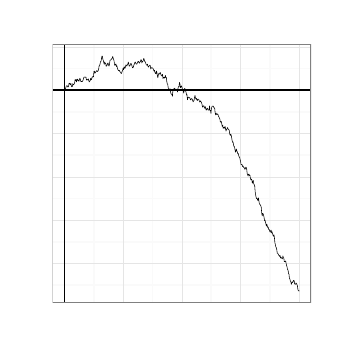
\begin{tikzpicture}[x=1pt,y=1pt]
\definecolor{fillColor}{RGB}{255,255,255}
\path[use as bounding box,fill=fillColor,fill opacity=0.00] (0,0) rectangle (108.41,108.41);
\begin{scope}
\path[clip] (  0.00,  0.00) rectangle (108.40,108.41);
\definecolor{drawColor}{RGB}{255,255,255}
\definecolor{fillColor}{RGB}{255,255,255}

\path[draw=drawColor,line width= 0.6pt,line join=round,line cap=round,fill=fillColor] (  0.00,  0.00) rectangle (108.41,108.41);
\end{scope}
\begin{scope}
\path[clip] (  9.00,  9.00) rectangle (102.41,102.41);
\definecolor{fillColor}{RGB}{255,255,255}

\path[fill=fillColor] (  9.00,  9.00) rectangle (102.40,102.41);
\definecolor{drawColor}{gray}{0.98}

\path[draw=drawColor,line width= 0.6pt,line join=round] (  9.00, 15.31) --
	(102.41, 15.31);

\path[draw=drawColor,line width= 0.6pt,line join=round] (  9.00, 30.97) --
	(102.41, 30.97);

\path[draw=drawColor,line width= 0.6pt,line join=round] (  9.00, 46.64) --
	(102.41, 46.64);

\path[draw=drawColor,line width= 0.6pt,line join=round] (  9.00, 62.30) --
	(102.41, 62.30);

\path[draw=drawColor,line width= 0.6pt,line join=round] (  9.00, 77.96) --
	(102.41, 77.96);

\path[draw=drawColor,line width= 0.6pt,line join=round] (  9.00, 93.63) --
	(102.41, 93.63);

\path[draw=drawColor,line width= 0.6pt,line join=round] ( 23.86,  9.00) --
	( 23.86,102.41);

\path[draw=drawColor,line width= 0.6pt,line join=round] ( 45.09,  9.00) --
	( 45.09,102.41);

\path[draw=drawColor,line width= 0.6pt,line join=round] ( 66.32,  9.00) --
	( 66.32,102.41);

\path[draw=drawColor,line width= 0.6pt,line join=round] ( 87.55,  9.00) --
	( 87.55,102.41);
\definecolor{drawColor}{gray}{0.90}

\path[draw=drawColor,line width= 0.2pt,line join=round] (  9.00, 23.14) --
	(102.41, 23.14);

\path[draw=drawColor,line width= 0.2pt,line join=round] (  9.00, 38.80) --
	(102.41, 38.80);

\path[draw=drawColor,line width= 0.2pt,line join=round] (  9.00, 54.47) --
	(102.41, 54.47);

\path[draw=drawColor,line width= 0.2pt,line join=round] (  9.00, 70.13) --
	(102.41, 70.13);

\path[draw=drawColor,line width= 0.2pt,line join=round] (  9.00, 85.80) --
	(102.41, 85.80);

\path[draw=drawColor,line width= 0.2pt,line join=round] (  9.00,101.46) --
	(102.41,101.46);

\path[draw=drawColor,line width= 0.2pt,line join=round] ( 13.25,  9.00) --
	( 13.25,102.41);

\path[draw=drawColor,line width= 0.2pt,line join=round] ( 34.47,  9.00) --
	( 34.47,102.41);

\path[draw=drawColor,line width= 0.2pt,line join=round] ( 55.70,  9.00) --
	( 55.70,102.41);

\path[draw=drawColor,line width= 0.2pt,line join=round] ( 76.93,  9.00) --
	( 76.93,102.41);

\path[draw=drawColor,line width= 0.2pt,line join=round] ( 98.16,  9.00) --
	( 98.16,102.41);
\definecolor{drawColor}{RGB}{0,0,0}

\path[draw=drawColor,line width= 0.2pt,line join=round] ( 13.25, 85.80) --
	( 13.42, 86.00) --
	( 13.59, 86.30) --
	( 13.76, 86.73) --
	( 13.92, 87.23) --
	( 14.09, 87.42) --
	( 14.26, 87.49) --
	( 14.43, 87.00) --
	( 14.60, 86.96) --
	( 14.77, 87.22) --
	( 14.94, 88.25) --
	( 15.11, 88.33) --
	( 15.28, 87.96) --
	( 15.45, 87.81) --
	( 15.62, 88.31) --
	( 15.79, 87.27) --
	( 15.96, 87.01) --
	( 16.13, 87.12) --
	( 16.30, 88.16) --
	( 16.47, 87.72) --
	( 16.64, 87.84) --
	( 16.81, 88.11) --
	( 16.98, 88.55) --
	( 17.15, 89.73) --
	( 17.32, 89.23) --
	( 17.49, 89.60) --
	( 17.66, 88.79) --
	( 17.83, 89.68) --
	( 18.00, 89.83) --
	( 18.17, 89.30) --
	( 18.34, 89.52) --
	( 18.51, 88.98) --
	( 18.68, 89.53) --
	( 18.85, 90.13) --
	( 19.02, 89.75) --
	( 19.19, 89.04) --
	( 19.36, 88.92) --
	( 19.53, 88.98) --
	( 19.70, 88.93) --
	( 19.87, 89.17) --
	( 20.04, 89.51) --
	( 20.21, 90.18) --
	( 20.38, 90.54) --
	( 20.55, 90.55) --
	( 20.72, 90.59) --
	( 20.89, 90.48) --
	( 21.06, 90.54) --
	( 21.23, 89.47) --
	( 21.40, 89.74) --
	( 21.57, 89.52) --
	( 21.74, 89.54) --
	( 21.91, 89.93) --
	( 22.08, 89.27) --
	( 22.25, 88.81) --
	( 22.42, 89.12) --
	( 22.59, 89.21) --
	( 22.76, 90.12) --
	( 22.93, 89.61) --
	( 23.10, 89.69) --
	( 23.27, 90.52) --
	( 23.44, 90.55) --
	( 23.61, 90.83) --
	( 23.77, 90.60) --
	( 23.94, 92.61) --
	( 24.11, 92.71) --
	( 24.28, 92.01) --
	( 24.45, 92.10) --
	( 24.62, 92.47) --
	( 24.79, 92.65) --
	( 24.96, 92.91) --
	( 25.13, 92.56) --
	( 25.30, 92.66) --
	( 25.47, 92.78) --
	( 25.64, 93.37) --
	( 25.81, 94.58) --
	( 25.98, 94.68) --
	( 26.15, 95.29) --
	( 26.32, 96.16) --
	( 26.49, 96.23) --
	( 26.66, 97.14) --
	( 26.83, 98.16) --
	( 27.00, 98.10) --
	( 27.17, 96.97) --
	( 27.34, 96.52) --
	( 27.51, 95.72) --
	( 27.68, 95.14) --
	( 27.85, 96.05) --
	( 28.02, 95.51) --
	( 28.19, 95.54) --
	( 28.36, 94.39) --
	( 28.53, 94.96) --
	( 28.70, 94.79) --
	( 28.87, 95.42) --
	( 29.04, 95.68) --
	( 29.21, 94.87) --
	( 29.38, 94.53) --
	( 29.55, 95.05) --
	( 29.72, 96.53) --
	( 29.89, 96.69) --
	( 30.06, 96.79) --
	( 30.23, 96.98) --
	( 30.40, 97.25) --
	( 30.57, 97.42) --
	( 30.74, 98.02) --
	( 30.91, 97.30) --
	( 31.08, 96.90) --
	( 31.25, 96.19) --
	( 31.42, 94.82) --
	( 31.59, 94.78) --
	( 31.76, 95.28) --
	( 31.93, 95.25) --
	( 32.10, 94.34) --
	( 32.27, 94.60) --
	( 32.44, 93.61) --
	( 32.61, 93.29) --
	( 32.78, 92.92) --
	( 32.95, 92.94) --
	( 33.12, 92.97) --
	( 33.29, 92.53) --
	( 33.46, 92.43) --
	( 33.62, 92.19) --
	( 33.79, 91.83) --
	( 33.96, 91.98) --
	( 34.13, 92.63) --
	( 34.30, 92.91) --
	( 34.47, 93.78) --
	( 34.64, 93.23) --
	( 34.81, 94.10) --
	( 34.98, 94.26) --
	( 35.15, 93.66) --
	( 35.32, 94.14) --
	( 35.49, 95.00) --
	( 35.66, 94.86) --
	( 35.83, 94.52) --
	( 36.00, 94.92) --
	( 36.17, 95.19) --
	( 36.34, 95.99) --
	( 36.51, 95.49) --
	( 36.68, 94.45) --
	( 36.85, 94.69) --
	( 37.02, 94.74) --
	( 37.19, 95.38) --
	( 37.36, 95.50) --
	( 37.53, 95.05) --
	( 37.70, 94.56) --
	( 37.87, 93.89) --
	( 38.04, 94.03) --
	( 38.21, 94.18) --
	( 38.38, 95.00) --
	( 38.55, 95.20) --
	( 38.72, 95.86) --
	( 38.89, 96.00) --
	( 39.06, 95.55) --
	( 39.23, 95.26) --
	( 39.40, 95.20) --
	( 39.57, 95.55) --
	( 39.74, 95.99) --
	( 39.91, 96.21) --
	( 40.08, 96.21) --
	( 40.25, 95.66) --
	( 40.42, 95.56) --
	( 40.59, 96.04) --
	( 40.76, 96.23) --
	( 40.93, 96.86) --
	( 41.10, 96.72) --
	( 41.27, 95.62) --
	( 41.44, 96.27) --
	( 41.61, 96.18) --
	( 41.78, 96.60) --
	( 41.95, 97.33) --
	( 42.12, 96.79) --
	( 42.29, 96.18) --
	( 42.46, 96.13) --
	( 42.63, 95.59) --
	( 42.80, 95.20) --
	( 42.97, 94.91) --
	( 43.14, 94.81) --
	( 43.31, 95.20) --
	( 43.47, 94.50) --
	( 43.64, 94.14) --
	( 43.81, 94.44) --
	( 43.98, 94.58) --
	( 44.15, 94.90) --
	( 44.32, 94.59) --
	( 44.49, 93.45) --
	( 44.66, 93.82) --
	( 44.83, 93.98) --
	( 45.00, 93.91) --
	( 45.17, 93.82) --
	( 45.34, 93.54) --
	( 45.51, 93.09) --
	( 45.68, 92.65) --
	( 45.85, 93.06) --
	( 46.02, 92.19) --
	( 46.19, 91.89) --
	( 46.36, 91.73) --
	( 46.53, 92.75) --
	( 46.70, 92.21) --
	( 46.87, 91.02) --
	( 47.04, 90.30) --
	( 47.21, 91.30) --
	( 47.38, 91.85) --
	( 47.55, 91.61) --
	( 47.72, 91.88) --
	( 47.89, 92.24) --
	( 48.06, 91.78) --
	( 48.23, 91.20) --
	( 48.40, 91.27) --
	( 48.57, 90.91) --
	( 48.74, 91.58) --
	( 48.91, 90.02) --
	( 49.08, 90.41) --
	( 49.25, 90.47) --
	( 49.42, 90.17) --
	( 49.59, 90.45) --
	( 49.76, 91.16) --
	( 49.93, 90.37) --
	( 50.10, 90.47) --
	( 50.27, 88.90) --
	( 50.44, 88.14) --
	( 50.61, 87.94) --
	( 50.78, 86.71) --
	( 50.95, 86.46) --
	( 51.12, 86.04) --
	( 51.29, 85.68) --
	( 51.46, 86.34) --
	( 51.63, 85.20) --
	( 51.80, 84.50) --
	( 51.97, 84.36) --
	( 52.14, 84.33) --
	( 52.31, 83.60) --
	( 52.48, 85.84) --
	( 52.65, 85.95) --
	( 52.82, 86.38) --
	( 52.99, 86.04) --
	( 53.16, 86.57) --
	( 53.32, 85.81) --
	( 53.49, 85.91) --
	( 53.66, 86.17) --
	( 53.83, 86.05) --
	( 54.00, 85.81) --
	( 54.17, 85.17) --
	( 54.34, 86.63) --
	( 54.51, 87.08) --
	( 54.68, 87.16) --
	( 54.85, 88.63) --
	( 55.02, 88.11) --
	( 55.19, 86.73) --
	( 55.36, 86.96) --
	( 55.53, 87.40) --
	( 55.70, 87.12) --
	( 55.87, 86.36) --
	( 56.04, 85.72) --
	( 56.21, 85.55) --
	( 56.38, 84.76) --
	( 56.55, 85.76) --
	( 56.72, 86.51) --
	( 56.89, 86.26) --
	( 57.06, 85.49) --
	( 57.23, 85.08) --
	( 57.40, 84.03) --
	( 57.57, 84.24) --
	( 57.74, 82.36) --
	( 57.91, 83.04) --
	( 58.08, 83.35) --
	( 58.25, 83.26) --
	( 58.42, 83.15) --
	( 58.59, 83.04) --
	( 58.76, 82.50) --
	( 58.93, 82.30) --
	( 59.10, 82.72) --
	( 59.27, 82.75) --
	( 59.44, 82.64) --
	( 59.61, 82.15) --
	( 59.78, 81.60) --
	( 59.95, 81.92) --
	( 60.12, 82.13) --
	( 60.29, 83.18) --
	( 60.46, 83.90) --
	( 60.63, 83.05) --
	( 60.80, 82.60) --
	( 60.97, 82.90) --
	( 61.14, 82.35) --
	( 61.31, 82.06) --
	( 61.48, 82.62) --
	( 61.65, 82.56) --
	( 61.82, 82.49) --
	( 61.99, 82.07) --
	( 62.16, 81.54) --
	( 62.33, 81.70) --
	( 62.50, 81.98) --
	( 62.67, 81.57) --
	( 62.84, 81.25) --
	( 63.01, 80.67) --
	( 63.17, 79.70) --
	( 63.34, 79.88) --
	( 63.51, 80.09) --
	( 63.68, 80.22) --
	( 63.85, 79.34) --
	( 64.02, 79.37) --
	( 64.19, 79.88) --
	( 64.36, 79.09) --
	( 64.53, 78.60) --
	( 64.70, 78.92) --
	( 64.87, 79.37) --
	( 65.04, 79.07) --
	( 65.21, 78.60) --
	( 65.38, 78.59) --
	( 65.55, 78.76) --
	( 65.72, 80.17) --
	( 65.89, 78.44) --
	( 66.06, 78.51) --
	( 66.23, 77.42) --
	( 66.40, 79.19) --
	( 66.57, 79.83) --
	( 66.74, 80.03) --
	( 66.91, 80.08) --
	( 67.08, 80.09) --
	( 67.25, 79.60) --
	( 67.42, 79.43) --
	( 67.59, 79.11) --
	( 67.76, 77.55) --
	( 67.93, 76.88) --
	( 68.10, 77.53) --
	( 68.27, 77.08) --
	( 68.44, 77.02) --
	( 68.61, 77.27) --
	( 68.78, 76.99) --
	( 68.95, 76.33) --
	( 69.12, 76.18) --
	( 69.29, 75.71) --
	( 69.46, 75.35) --
	( 69.63, 74.25) --
	( 69.80, 74.47) --
	( 69.97, 74.50) --
	( 70.14, 73.58) --
	( 70.31, 72.71) --
	( 70.48, 73.17) --
	( 70.65, 71.98) --
	( 70.82, 72.40) --
	( 70.99, 72.42) --
	( 71.16, 72.06) --
	( 71.33, 72.74) --
	( 71.50, 71.94) --
	( 71.67, 71.07) --
	( 71.84, 71.55) --
	( 72.01, 71.78) --
	( 72.18, 72.34) --
	( 72.35, 72.01) --
	( 72.52, 71.64) --
	( 72.69, 71.57) --
	( 72.86, 71.22) --
	( 73.02, 69.95) --
	( 73.19, 69.53) --
	( 73.36, 69.93) --
	( 73.53, 69.57) --
	( 73.70, 68.69) --
	( 73.87, 67.63) --
	( 74.04, 66.97) --
	( 74.21, 67.14) --
	( 74.38, 66.13) --
	( 74.55, 65.44) --
	( 74.72, 65.44) --
	( 74.89, 64.44) --
	( 75.06, 63.44) --
	( 75.23, 63.75) --
	( 75.40, 64.58) --
	( 75.57, 63.92) --
	( 75.74, 63.58) --
	( 75.91, 62.83) --
	( 76.08, 62.97) --
	( 76.25, 62.17) --
	( 76.42, 61.71) --
	( 76.59, 61.63) --
	( 76.76, 60.75) --
	( 76.93, 60.11) --
	( 77.10, 58.95) --
	( 77.27, 58.88) --
	( 77.44, 58.99) --
	( 77.61, 58.21) --
	( 77.78, 58.48) --
	( 77.95, 58.18) --
	( 78.12, 57.83) --
	( 78.29, 57.85) --
	( 78.46, 57.25) --
	( 78.63, 57.31) --
	( 78.80, 58.03) --
	( 78.97, 57.95) --
	( 79.14, 57.34) --
	( 79.31, 55.75) --
	( 79.48, 55.27) --
	( 79.65, 54.75) --
	( 79.82, 55.53) --
	( 79.99, 55.44) --
	( 80.16, 54.99) --
	( 80.33, 55.00) --
	( 80.50, 53.83) --
	( 80.67, 53.41) --
	( 80.84, 53.72) --
	( 81.01, 53.37) --
	( 81.18, 52.20) --
	( 81.35, 52.78) --
	( 81.52, 53.21) --
	( 81.69, 52.00) --
	( 81.86, 51.68) --
	( 82.03, 51.34) --
	( 82.20, 49.16) --
	( 82.37, 47.98) --
	( 82.54, 47.14) --
	( 82.71, 46.65) --
	( 82.87, 46.80) --
	( 83.04, 46.25) --
	( 83.21, 45.95) --
	( 83.38, 46.91) --
	( 83.55, 45.83) --
	( 83.72, 44.81) --
	( 83.89, 44.55) --
	( 84.06, 44.37) --
	( 84.23, 44.08) --
	( 84.40, 43.48) --
	( 84.57, 41.40) --
	( 84.74, 40.38) --
	( 84.91, 41.35) --
	( 85.08, 41.14) --
	( 85.25, 40.57) --
	( 85.42, 39.92) --
	( 85.59, 38.62) --
	( 85.76, 38.89) --
	( 85.93, 38.16) --
	( 86.10, 37.40) --
	( 86.27, 36.68) --
	( 86.44, 37.39) --
	( 86.61, 36.71) --
	( 86.78, 36.08) --
	( 86.95, 36.34) --
	( 87.12, 35.41) --
	( 87.29, 35.52) --
	( 87.46, 34.92) --
	( 87.63, 34.48) --
	( 87.80, 35.10) --
	( 87.97, 35.27) --
	( 88.14, 34.20) --
	( 88.31, 34.66) --
	( 88.48, 34.01) --
	( 88.65, 33.43) --
	( 88.82, 33.05) --
	( 88.99, 33.56) --
	( 89.16, 32.53) --
	( 89.33, 30.69) --
	( 89.50, 30.05) --
	( 89.67, 29.18) --
	( 89.84, 28.95) --
	( 90.01, 28.17) --
	( 90.18, 26.92) --
	( 90.35, 26.92) --
	( 90.52, 26.60) --
	( 90.69, 26.18) --
	( 90.86, 26.07) --
	( 91.03, 25.73) --
	( 91.20, 26.11) --
	( 91.37, 25.18) --
	( 91.54, 25.48) --
	( 91.71, 25.20) --
	( 91.88, 25.04) --
	( 92.05, 24.89) --
	( 92.22, 25.96) --
	( 92.39, 25.23) --
	( 92.56, 25.17) --
	( 92.72, 23.89) --
	( 92.89, 23.89) --
	( 93.06, 23.95) --
	( 93.23, 24.10) --
	( 93.40, 23.18) --
	( 93.57, 22.41) --
	( 93.74, 21.91) --
	( 93.91, 20.90) --
	( 94.08, 20.86) --
	( 94.25, 19.70) --
	( 94.42, 19.31) --
	( 94.59, 17.88) --
	( 94.76, 17.58) --
	( 94.93, 16.83) --
	( 95.10, 16.62) --
	( 95.27, 15.62) --
	( 95.44, 16.26) --
	( 95.61, 16.51) --
	( 95.78, 16.32) --
	( 95.95, 16.85) --
	( 96.12, 17.11) --
	( 96.29, 17.00) --
	( 96.46, 15.79) --
	( 96.63, 15.76) --
	( 96.80, 15.68) --
	( 96.97, 16.16) --
	( 97.14, 15.91) --
	( 97.31, 15.53) --
	( 97.48, 15.15) --
	( 97.65, 13.63) --
	( 97.82, 13.54) --
	( 97.99, 13.25) --
	( 98.16, 13.36);

\path[draw=drawColor,line width= 0.6pt,line join=round] (  9.00, 85.80) -- (102.41, 85.80);

\path[draw=drawColor,line width= 0.6pt,line join=round] ( 13.25,  9.00) -- ( 13.25,102.41);
\definecolor{drawColor}{gray}{0.50}

\path[draw=drawColor,line width= 0.6pt,line join=round,line cap=round] (  9.00,  9.00) rectangle (102.40,102.41);
\end{scope}
\end{tikzpicture}
}%
	\quad
	\subfloat[$B^{\pp_1}(s)$]{% Created by tikzDevice version 0.10.1 on 2017-01-16 15:57:32
% !TEX encoding = UTF-8 Unicode
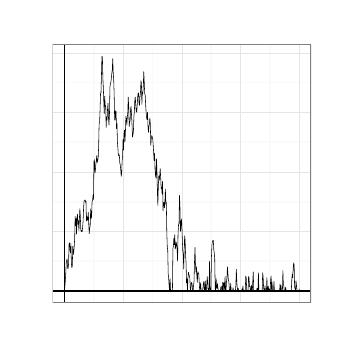
\begin{tikzpicture}[x=1pt,y=1pt]
\definecolor{fillColor}{RGB}{255,255,255}
\path[use as bounding box,fill=fillColor,fill opacity=0.00] (0,0) rectangle (108.41,108.41);
\begin{scope}
\path[clip] (  0.00,  0.00) rectangle (108.40,108.41);
\definecolor{drawColor}{RGB}{255,255,255}
\definecolor{fillColor}{RGB}{255,255,255}

\path[draw=drawColor,line width= 0.6pt,line join=round,line cap=round,fill=fillColor] (  0.00,  0.00) rectangle (108.41,108.41);
\end{scope}
\begin{scope}
\path[clip] (  9.00,  9.00) rectangle (102.41,102.41);
\definecolor{fillColor}{RGB}{255,255,255}

\path[fill=fillColor] (  9.00,  9.00) rectangle (102.40,102.41);
\definecolor{drawColor}{gray}{0.98}

\path[draw=drawColor,line width= 0.6pt,line join=round] (  9.00, 24.00) --
	(102.41, 24.00);

\path[draw=drawColor,line width= 0.6pt,line join=round] (  9.00, 45.52) --
	(102.41, 45.52);

\path[draw=drawColor,line width= 0.6pt,line join=round] (  9.00, 67.03) --
	(102.41, 67.03);

\path[draw=drawColor,line width= 0.6pt,line join=round] (  9.00, 88.55) --
	(102.41, 88.55);

\path[draw=drawColor,line width= 0.6pt,line join=round] ( 23.86,  9.00) --
	( 23.86,102.41);

\path[draw=drawColor,line width= 0.6pt,line join=round] ( 45.09,  9.00) --
	( 45.09,102.41);

\path[draw=drawColor,line width= 0.6pt,line join=round] ( 66.32,  9.00) --
	( 66.32,102.41);

\path[draw=drawColor,line width= 0.6pt,line join=round] ( 87.55,  9.00) --
	( 87.55,102.41);
\definecolor{drawColor}{gray}{0.90}

\path[draw=drawColor,line width= 0.2pt,line join=round] (  9.00, 13.25) --
	(102.41, 13.25);

\path[draw=drawColor,line width= 0.2pt,line join=round] (  9.00, 34.76) --
	(102.41, 34.76);

\path[draw=drawColor,line width= 0.2pt,line join=round] (  9.00, 56.28) --
	(102.41, 56.28);

\path[draw=drawColor,line width= 0.2pt,line join=round] (  9.00, 77.79) --
	(102.41, 77.79);

\path[draw=drawColor,line width= 0.2pt,line join=round] (  9.00, 99.31) --
	(102.41, 99.31);

\path[draw=drawColor,line width= 0.2pt,line join=round] ( 13.25,  9.00) --
	( 13.25,102.41);

\path[draw=drawColor,line width= 0.2pt,line join=round] ( 34.47,  9.00) --
	( 34.47,102.41);

\path[draw=drawColor,line width= 0.2pt,line join=round] ( 55.70,  9.00) --
	( 55.70,102.41);

\path[draw=drawColor,line width= 0.2pt,line join=round] ( 76.93,  9.00) --
	( 76.93,102.41);

\path[draw=drawColor,line width= 0.2pt,line join=round] ( 98.16,  9.00) --
	( 98.16,102.41);
\definecolor{drawColor}{RGB}{0,0,0}

\path[draw=drawColor,line width= 0.2pt,line join=round] ( 13.25, 13.25) --
	( 13.42, 14.68) --
	( 13.59, 16.72) --
	( 13.76, 19.63) --
	( 13.92, 23.08) --
	( 14.09, 24.38) --
	( 14.26, 24.91) --
	( 14.43, 21.54) --
	( 14.60, 21.27) --
	( 14.77, 23.00) --
	( 14.94, 30.10) --
	( 15.11, 30.66) --
	( 15.28, 28.11) --
	( 15.45, 27.06) --
	( 15.62, 30.50) --
	( 15.79, 23.39) --
	( 15.96, 21.62) --
	( 16.13, 22.37) --
	( 16.30, 29.50) --
	( 16.47, 26.45) --
	( 16.64, 27.29) --
	( 16.81, 29.14) --
	( 16.98, 32.18) --
	( 17.15, 40.25) --
	( 17.32, 36.80) --
	( 17.49, 39.36) --
	( 17.66, 33.78) --
	( 17.83, 39.96) --
	( 18.00, 40.96) --
	( 18.17, 37.32) --
	( 18.34, 38.80) --
	( 18.51, 35.11) --
	( 18.68, 38.93) --
	( 18.85, 42.98) --
	( 19.02, 40.42) --
	( 19.19, 35.55) --
	( 19.36, 34.72) --
	( 19.53, 35.12) --
	( 19.70, 34.76) --
	( 19.87, 36.44) --
	( 20.04, 38.77) --
	( 20.21, 43.38) --
	( 20.38, 45.81) --
	( 20.55, 45.90) --
	( 20.72, 46.16) --
	( 20.89, 45.44) --
	( 21.06, 45.85) --
	( 21.23, 38.50) --
	( 21.40, 40.36) --
	( 21.57, 38.85) --
	( 21.74, 38.94) --
	( 21.91, 41.67) --
	( 22.08, 37.10) --
	( 22.25, 33.98) --
	( 22.42, 36.09) --
	( 22.59, 36.72) --
	( 22.76, 42.95) --
	( 22.93, 39.46) --
	( 23.10, 39.99) --
	( 23.27, 45.72) --
	( 23.44, 45.88) --
	( 23.61, 47.79) --
	( 23.77, 46.24) --
	( 23.94, 60.07) --
	( 24.11, 60.74) --
	( 24.28, 55.94) --
	( 24.45, 56.57) --
	( 24.62, 59.09) --
	( 24.79, 60.30) --
	( 24.96, 62.12) --
	( 25.13, 59.70) --
	( 25.30, 60.37) --
	( 25.47, 61.23) --
	( 25.64, 65.29) --
	( 25.81, 73.57) --
	( 25.98, 74.26) --
	( 26.15, 78.48) --
	( 26.32, 84.46) --
	( 26.49, 84.89) --
	( 26.66, 91.18) --
	( 26.83, 98.16) --
	( 27.00, 97.72) --
	( 27.17, 89.97) --
	( 27.34, 86.93) --
	( 27.51, 81.44) --
	( 27.68, 77.39) --
	( 27.85, 83.64) --
	( 28.02, 79.96) --
	( 28.19, 80.20) --
	( 28.36, 72.30) --
	( 28.53, 76.16) --
	( 28.70, 75.02) --
	( 28.87, 79.35) --
	( 29.04, 81.15) --
	( 29.21, 75.60) --
	( 29.38, 73.25) --
	( 29.55, 76.78) --
	( 29.72, 86.95) --
	( 29.89, 88.08) --
	( 30.06, 88.73) --
	( 30.23, 90.08) --
	( 30.40, 91.93) --
	( 30.57, 93.09) --
	( 30.74, 97.20) --
	( 30.91, 92.25) --
	( 31.08, 89.54) --
	( 31.25, 84.64) --
	( 31.42, 75.20) --
	( 31.59, 74.93) --
	( 31.76, 78.41) --
	( 31.93, 78.19) --
	( 32.10, 71.96) --
	( 32.27, 73.70) --
	( 32.44, 66.91) --
	( 32.61, 64.69) --
	( 32.78, 62.18) --
	( 32.95, 62.33) --
	( 33.12, 62.50) --
	( 33.29, 59.48) --
	( 33.46, 58.84) --
	( 33.62, 57.17) --
	( 33.79, 54.70) --
	( 33.96, 55.74) --
	( 34.13, 60.21) --
	( 34.30, 62.11) --
	( 34.47, 68.11) --
	( 34.64, 64.27) --
	( 34.81, 70.28) --
	( 34.98, 71.38) --
	( 35.15, 67.24) --
	( 35.32, 70.53) --
	( 35.49, 76.48) --
	( 35.66, 75.51) --
	( 35.83, 73.15) --
	( 36.00, 75.88) --
	( 36.17, 77.78) --
	( 36.34, 83.27) --
	( 36.51, 79.83) --
	( 36.68, 72.67) --
	( 36.85, 74.35) --
	( 37.02, 74.65) --
	( 37.19, 79.04) --
	( 37.36, 79.93) --
	( 37.53, 76.83) --
	( 37.70, 73.44) --
	( 37.87, 68.85) --
	( 38.04, 69.77) --
	( 38.21, 70.80) --
	( 38.38, 76.44) --
	( 38.55, 77.87) --
	( 38.72, 82.39) --
	( 38.89, 83.31) --
	( 39.06, 80.25) --
	( 39.23, 78.26) --
	( 39.40, 77.81) --
	( 39.57, 80.23) --
	( 39.74, 83.24) --
	( 39.91, 84.79) --
	( 40.08, 84.81) --
	( 40.25, 80.97) --
	( 40.42, 80.33) --
	( 40.59, 83.59) --
	( 40.76, 84.91) --
	( 40.93, 89.25) --
	( 41.10, 88.31) --
	( 41.27, 80.70) --
	( 41.44, 85.15) --
	( 41.61, 84.60) --
	( 41.78, 87.42) --
	( 41.95, 92.50) --
	( 42.12, 88.74) --
	( 42.29, 84.56) --
	( 42.46, 84.22) --
	( 42.63, 80.53) --
	( 42.80, 77.81) --
	( 42.97, 75.86) --
	( 43.14, 75.15) --
	( 43.31, 77.80) --
	( 43.47, 73.04) --
	( 43.64, 70.59) --
	( 43.81, 72.60) --
	( 43.98, 73.56) --
	( 44.15, 75.76) --
	( 44.32, 73.65) --
	( 44.49, 65.83) --
	( 44.66, 68.37) --
	( 44.83, 69.43) --
	( 45.00, 68.97) --
	( 45.17, 68.33) --
	( 45.34, 66.43) --
	( 45.51, 63.32) --
	( 45.68, 60.35) --
	( 45.85, 63.11) --
	( 46.02, 57.19) --
	( 46.19, 55.12) --
	( 46.36, 54.02) --
	( 46.53, 61.03) --
	( 46.70, 57.31) --
	( 46.87, 49.13) --
	( 47.04, 44.20) --
	( 47.21, 51.02) --
	( 47.38, 54.85) --
	( 47.55, 53.21) --
	( 47.72, 55.01) --
	( 47.89, 57.48) --
	( 48.06, 54.35) --
	( 48.23, 50.34) --
	( 48.40, 50.83) --
	( 48.57, 48.40) --
	( 48.74, 52.97) --
	( 48.91, 42.27) --
	( 49.08, 44.92) --
	( 49.25, 45.33) --
	( 49.42, 43.27) --
	( 49.59, 45.24) --
	( 49.76, 50.06) --
	( 49.93, 44.65) --
	( 50.10, 45.36) --
	( 50.27, 34.57) --
	( 50.44, 29.36) --
	( 50.61, 27.97) --
	( 50.78, 19.49) --
	( 50.95, 17.80) --
	( 51.12, 14.92) --
	( 51.29, 13.25) --
	( 51.46, 17.75) --
	( 51.63, 13.25) --
	( 51.80, 13.25) --
	( 51.97, 13.25) --
	( 52.14, 13.25) --
	( 52.31, 13.25) --
	( 52.48, 28.63) --
	( 52.65, 29.39) --
	( 52.82, 32.33) --
	( 52.99, 29.98) --
	( 53.16, 33.63) --
	( 53.32, 28.45) --
	( 53.49, 29.13) --
	( 53.66, 30.89) --
	( 53.83, 30.03) --
	( 54.00, 28.38) --
	( 54.17, 24.03) --
	( 54.34, 34.06) --
	( 54.51, 37.11) --
	( 54.68, 37.69) --
	( 54.85, 47.78) --
	( 55.02, 44.22) --
	( 55.19, 34.75) --
	( 55.36, 36.28) --
	( 55.53, 39.33) --
	( 55.70, 37.42) --
	( 55.87, 32.20) --
	( 56.04, 27.77) --
	( 56.21, 26.64) --
	( 56.38, 21.19) --
	( 56.55, 28.07) --
	( 56.72, 33.24) --
	( 56.89, 31.53) --
	( 57.06, 26.22) --
	( 57.23, 23.43) --
	( 57.40, 16.20) --
	( 57.57, 17.61) --
	( 57.74, 13.25) --
	( 57.91, 17.92) --
	( 58.08, 20.02) --
	( 58.25, 19.40) --
	( 58.42, 18.64) --
	( 58.59, 17.90) --
	( 58.76, 14.21) --
	( 58.93, 13.25) --
	( 59.10, 16.08) --
	( 59.27, 16.33) --
	( 59.44, 15.55) --
	( 59.61, 13.25) --
	( 59.78, 13.25) --
	( 59.95, 15.43) --
	( 60.12, 16.86) --
	( 60.29, 24.05) --
	( 60.46, 28.98) --
	( 60.63, 23.19) --
	( 60.80, 20.11) --
	( 60.97, 22.13) --
	( 61.14, 18.38) --
	( 61.31, 16.39) --
	( 61.48, 20.25) --
	( 61.65, 19.84) --
	( 61.82, 19.36) --
	( 61.99, 16.47) --
	( 62.16, 13.25) --
	( 62.33, 14.34) --
	( 62.50, 16.26) --
	( 62.67, 13.47) --
	( 62.84, 13.25) --
	( 63.01, 13.25) --
	( 63.17, 13.25) --
	( 63.34, 14.46) --
	( 63.51, 15.95) --
	( 63.68, 16.79) --
	( 63.85, 13.25) --
	( 64.02, 13.46) --
	( 64.19, 16.91) --
	( 64.36, 13.25) --
	( 64.53, 13.25) --
	( 64.70, 15.39) --
	( 64.87, 18.50) --
	( 65.04, 16.44) --
	( 65.21, 13.25) --
	( 65.38, 13.25) --
	( 65.55, 14.38) --
	( 65.72, 24.10) --
	( 65.89, 13.25) --
	( 66.06, 13.75) --
	( 66.23, 13.25) --
	( 66.40, 25.36) --
	( 66.57, 29.76) --
	( 66.74, 31.14) --
	( 66.91, 31.50) --
	( 67.08, 31.55) --
	( 67.25, 28.19) --
	( 67.42, 27.05) --
	( 67.59, 24.83) --
	( 67.76, 14.15) --
	( 67.93, 13.25) --
	( 68.10, 17.74) --
	( 68.27, 14.59) --
	( 68.44, 14.22) --
	( 68.61, 15.94) --
	( 68.78, 14.03) --
	( 68.95, 13.25) --
	( 69.12, 13.25) --
	( 69.29, 13.25) --
	( 69.46, 13.25) --
	( 69.63, 13.25) --
	( 69.80, 14.75) --
	( 69.97, 14.95) --
	( 70.14, 13.25) --
	( 70.31, 13.25) --
	( 70.48, 16.41) --
	( 70.65, 13.25) --
	( 70.82, 16.12) --
	( 70.99, 16.27) --
	( 71.16, 13.79) --
	( 71.33, 18.51) --
	( 71.50, 13.25) --
	( 71.67, 13.25) --
	( 71.84, 16.58) --
	( 72.01, 18.16) --
	( 72.18, 22.02) --
	( 72.35, 19.69) --
	( 72.52, 17.19) --
	( 72.69, 16.73) --
	( 72.86, 14.32) --
	( 73.02, 13.25) --
	( 73.19, 13.25) --
	( 73.36, 15.99) --
	( 73.53, 13.53) --
	( 73.70, 13.25) --
	( 73.87, 13.25) --
	( 74.04, 13.25) --
	( 74.21, 14.45) --
	( 74.38, 13.25) --
	( 74.55, 13.25) --
	( 74.72, 13.25) --
	( 74.89, 13.25) --
	( 75.06, 13.25) --
	( 75.23, 15.39) --
	( 75.40, 21.08) --
	( 75.57, 16.53) --
	( 75.74, 14.24) --
	( 75.91, 13.25) --
	( 76.08, 14.18) --
	( 76.25, 13.25) --
	( 76.42, 13.25) --
	( 76.59, 13.25) --
	( 76.76, 13.25) --
	( 76.93, 13.25) --
	( 77.10, 13.25) --
	( 77.27, 13.25) --
	( 77.44, 14.01) --
	( 77.61, 13.25) --
	( 77.78, 15.10) --
	( 77.95, 13.25) --
	( 78.12, 13.25) --
	( 78.29, 13.35) --
	( 78.46, 13.25) --
	( 78.63, 13.61) --
	( 78.80, 18.59) --
	( 78.97, 17.99) --
	( 79.14, 13.86) --
	( 79.31, 13.25) --
	( 79.48, 13.25) --
	( 79.65, 13.25) --
	( 79.82, 18.57) --
	( 79.99, 17.98) --
	( 80.16, 14.88) --
	( 80.33, 14.95) --
	( 80.50, 13.25) --
	( 80.67, 13.25) --
	( 80.84, 15.43) --
	( 81.01, 13.25) --
	( 81.18, 13.25) --
	( 81.35, 17.19) --
	( 81.52, 20.19) --
	( 81.69, 13.25) --
	( 81.86, 13.25) --
	( 82.03, 13.25) --
	( 82.20, 13.25) --
	( 82.37, 13.25) --
	( 82.54, 13.25) --
	( 82.71, 13.25) --
	( 82.87, 14.27) --
	( 83.04, 13.25) --
	( 83.21, 13.25) --
	( 83.38, 19.84) --
	( 83.55, 13.25) --
	( 83.72, 13.25) --
	( 83.89, 13.25) --
	( 84.06, 13.25) --
	( 84.23, 13.25) --
	( 84.40, 13.25) --
	( 84.57, 13.25) --
	( 84.74, 13.25) --
	( 84.91, 19.85) --
	( 85.08, 18.46) --
	( 85.25, 14.55) --
	( 85.42, 13.25) --
	( 85.59, 13.25) --
	( 85.76, 15.11) --
	( 85.93, 13.25) --
	( 86.10, 13.25) --
	( 86.27, 13.25) --
	( 86.44, 18.15) --
	( 86.61, 13.48) --
	( 86.78, 13.25) --
	( 86.95, 15.06) --
	( 87.12, 13.25) --
	( 87.29, 13.99) --
	( 87.46, 13.25) --
	( 87.63, 13.25) --
	( 87.80, 17.50) --
	( 87.97, 18.67) --
	( 88.14, 13.25) --
	( 88.31, 16.36) --
	( 88.48, 13.25) --
	( 88.65, 13.25) --
	( 88.82, 13.25) --
	( 88.99, 16.76) --
	( 89.16, 13.25) --
	( 89.33, 13.25) --
	( 89.50, 13.25) --
	( 89.67, 13.25) --
	( 89.84, 13.25) --
	( 90.01, 13.25) --
	( 90.18, 13.25) --
	( 90.35, 13.26) --
	( 90.52, 13.25) --
	( 90.69, 13.25) --
	( 90.86, 13.25) --
	( 91.03, 13.25) --
	( 91.20, 15.83) --
	( 91.37, 13.25) --
	( 91.54, 15.27) --
	( 91.71, 13.36) --
	( 91.88, 13.25) --
	( 92.05, 13.25) --
	( 92.22, 20.61) --
	( 92.39, 15.61) --
	( 92.56, 15.20) --
	( 92.72, 13.25) --
	( 92.89, 13.25) --
	( 93.06, 13.66) --
	( 93.23, 14.69) --
	( 93.40, 13.25) --
	( 93.57, 13.25) --
	( 93.74, 13.25) --
	( 93.91, 13.25) --
	( 94.08, 13.25) --
	( 94.25, 13.25) --
	( 94.42, 13.25) --
	( 94.59, 13.25) --
	( 94.76, 13.25) --
	( 94.93, 13.25) --
	( 95.10, 13.25) --
	( 95.27, 13.25) --
	( 95.44, 17.61) --
	( 95.61, 19.35) --
	( 95.78, 18.04) --
	( 95.95, 21.70) --
	( 96.12, 23.43) --
	( 96.29, 22.71) --
	( 96.46, 14.43) --
	( 96.63, 14.22) --
	( 96.80, 13.66) --
	( 96.97, 16.93) --
	( 97.14, 15.20) --
	( 97.31, 13.25) --
	( 97.48, 13.25) --
	( 97.65, 13.25) --
	( 97.82, 13.25) --
	( 97.99, 13.25) --
	( 98.16, 14.05);

\path[draw=drawColor,line width= 0.6pt,line join=round] (  9.00, 13.25) -- (102.41, 13.25);

\path[draw=drawColor,line width= 0.6pt,line join=round] ( 13.25,  9.00) -- ( 13.25,102.41);
\definecolor{drawColor}{gray}{0.50}

\path[draw=drawColor,line width= 0.6pt,line join=round,line cap=round] (  9.00,  9.00) rectangle (102.40,102.41);
\end{scope}
\end{tikzpicture}
}%
	\quad
	\subfloat[$W^{\pp_2}(s)$]{% Created by tikzDevice version 0.10.1 on 2017-01-16 15:57:32
% !TEX encoding = UTF-8 Unicode
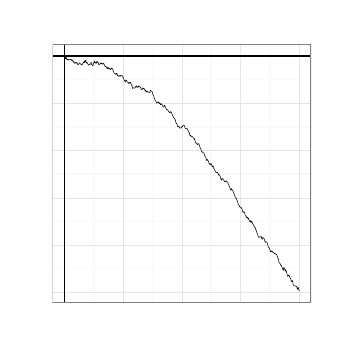
\begin{tikzpicture}[x=1pt,y=1pt]
\definecolor{fillColor}{RGB}{255,255,255}
\path[use as bounding box,fill=fillColor,fill opacity=0.00] (0,0) rectangle (108.41,108.41);
\begin{scope}
\path[clip] (  0.00,  0.00) rectangle (108.40,108.41);
\definecolor{drawColor}{RGB}{255,255,255}
\definecolor{fillColor}{RGB}{255,255,255}

\path[draw=drawColor,line width= 0.6pt,line join=round,line cap=round,fill=fillColor] (  0.00,  0.00) rectangle (108.41,108.41);
\end{scope}
\begin{scope}
\path[clip] (  9.00,  9.00) rectangle (102.41,102.41);
\definecolor{fillColor}{RGB}{255,255,255}

\path[fill=fillColor] (  9.00,  9.00) rectangle (102.40,102.41);
\definecolor{drawColor}{gray}{0.98}

\path[draw=drawColor,line width= 0.6pt,line join=round] (  9.00, 21.33) --
	(102.41, 21.33);

\path[draw=drawColor,line width= 0.6pt,line join=round] (  9.00, 38.40) --
	(102.41, 38.40);

\path[draw=drawColor,line width= 0.6pt,line join=round] (  9.00, 55.48) --
	(102.41, 55.48);

\path[draw=drawColor,line width= 0.6pt,line join=round] (  9.00, 72.55) --
	(102.41, 72.55);

\path[draw=drawColor,line width= 0.6pt,line join=round] (  9.00, 89.62) --
	(102.41, 89.62);

\path[draw=drawColor,line width= 0.6pt,line join=round] ( 23.86,  9.00) --
	( 23.86,102.41);

\path[draw=drawColor,line width= 0.6pt,line join=round] ( 45.09,  9.00) --
	( 45.09,102.41);

\path[draw=drawColor,line width= 0.6pt,line join=round] ( 66.32,  9.00) --
	( 66.32,102.41);

\path[draw=drawColor,line width= 0.6pt,line join=round] ( 87.55,  9.00) --
	( 87.55,102.41);
\definecolor{drawColor}{gray}{0.90}

\path[draw=drawColor,line width= 0.2pt,line join=round] (  9.00, 12.79) --
	(102.41, 12.79);

\path[draw=drawColor,line width= 0.2pt,line join=round] (  9.00, 29.87) --
	(102.41, 29.87);

\path[draw=drawColor,line width= 0.2pt,line join=round] (  9.00, 46.94) --
	(102.41, 46.94);

\path[draw=drawColor,line width= 0.2pt,line join=round] (  9.00, 64.01) --
	(102.41, 64.01);

\path[draw=drawColor,line width= 0.2pt,line join=round] (  9.00, 81.09) --
	(102.41, 81.09);

\path[draw=drawColor,line width= 0.2pt,line join=round] (  9.00, 98.16) --
	(102.41, 98.16);

\path[draw=drawColor,line width= 0.2pt,line join=round] ( 13.25,  9.00) --
	( 13.25,102.41);

\path[draw=drawColor,line width= 0.2pt,line join=round] ( 34.47,  9.00) --
	( 34.47,102.41);

\path[draw=drawColor,line width= 0.2pt,line join=round] ( 55.70,  9.00) --
	( 55.70,102.41);

\path[draw=drawColor,line width= 0.2pt,line join=round] ( 76.93,  9.00) --
	( 76.93,102.41);

\path[draw=drawColor,line width= 0.2pt,line join=round] ( 98.16,  9.00) --
	( 98.16,102.41);
\definecolor{drawColor}{RGB}{0,0,0}

\path[draw=drawColor,line width= 0.2pt,line join=round] ( 13.25, 98.16) --
	( 13.42, 98.03) --
	( 13.59, 97.37) --
	( 13.76, 97.11) --
	( 13.92, 97.90) --
	( 14.09, 97.19) --
	( 14.26, 96.82) --
	( 14.43, 96.92) --
	( 14.60, 96.78) --
	( 14.77, 96.66) --
	( 14.94, 97.00) --
	( 15.11, 96.94) --
	( 15.28, 97.00) --
	( 15.45, 97.01) --
	( 15.62, 96.92) --
	( 15.79, 96.55) --
	( 15.96, 96.84) --
	( 16.13, 96.73) --
	( 16.30, 96.43) --
	( 16.47, 95.97) --
	( 16.64, 96.19) --
	( 16.81, 95.62) --
	( 16.98, 95.54) --
	( 17.15, 95.82) --
	( 17.32, 95.61) --
	( 17.49, 95.92) --
	( 17.66, 95.58) --
	( 17.83, 95.82) --
	( 18.00, 95.25) --
	( 18.17, 95.07) --
	( 18.34, 95.15) --
	( 18.51, 95.35) --
	( 18.68, 95.60) --
	( 18.85, 95.67) --
	( 19.02, 95.23) --
	( 19.19, 95.28) --
	( 19.36, 95.02) --
	( 19.53, 95.00) --
	( 19.70, 94.99) --
	( 19.87, 95.39) --
	( 20.04, 95.58) --
	( 20.21, 96.04) --
	( 20.38, 95.74) --
	( 20.55, 96.42) --
	( 20.72, 95.90) --
	( 20.89, 96.62) --
	( 21.06, 96.41) --
	( 21.23, 95.65) --
	( 21.40, 95.86) --
	( 21.57, 95.77) --
	( 21.74, 95.31) --
	( 21.91, 95.10) --
	( 22.08, 94.82) --
	( 22.25, 94.99) --
	( 22.42, 95.20) --
	( 22.59, 95.28) --
	( 22.76, 95.24) --
	( 22.93, 95.99) --
	( 23.10, 95.10) --
	( 23.27, 94.95) --
	( 23.44, 94.68) --
	( 23.61, 94.74) --
	( 23.77, 95.47) --
	( 23.94, 95.94) --
	( 24.11, 96.32) --
	( 24.28, 95.63) --
	( 24.45, 95.87) --
	( 24.62, 95.61) --
	( 24.79, 95.46) --
	( 24.96, 96.27) --
	( 25.13, 96.24) --
	( 25.30, 95.80) --
	( 25.47, 95.95) --
	( 25.64, 95.10) --
	( 25.81, 94.99) --
	( 25.98, 95.23) --
	( 26.15, 95.30) --
	( 26.32, 95.59) --
	( 26.49, 95.55) --
	( 26.66, 95.29) --
	( 26.83, 95.73) --
	( 27.00, 95.21) --
	( 27.17, 95.23) --
	( 27.34, 95.44) --
	( 27.51, 95.49) --
	( 27.68, 95.06) --
	( 27.85, 94.69) --
	( 28.02, 94.39) --
	( 28.19, 94.35) --
	( 28.36, 94.32) --
	( 28.53, 94.14) --
	( 28.70, 93.59) --
	( 28.87, 93.65) --
	( 29.04, 94.25) --
	( 29.21, 93.66) --
	( 29.38, 93.53) --
	( 29.55, 93.68) --
	( 29.72, 93.60) --
	( 29.89, 93.20) --
	( 30.06, 93.58) --
	( 30.23, 93.61) --
	( 30.40, 93.86) --
	( 30.57, 93.47) --
	( 30.74, 93.55) --
	( 30.91, 92.66) --
	( 31.08, 92.41) --
	( 31.25, 91.95) --
	( 31.42, 91.86) --
	( 31.59, 91.92) --
	( 31.76, 91.52) --
	( 31.93, 91.54) --
	( 32.10, 91.84) --
	( 32.27, 91.88) --
	( 32.44, 91.00) --
	( 32.61, 91.07) --
	( 32.78, 91.09) --
	( 32.95, 90.81) --
	( 33.12, 90.86) --
	( 33.29, 91.16) --
	( 33.46, 91.11) --
	( 33.62, 90.86) --
	( 33.79, 91.10) --
	( 33.96, 91.10) --
	( 34.13, 90.88) --
	( 34.30, 91.00) --
	( 34.47, 90.40) --
	( 34.64, 90.26) --
	( 34.81, 89.49) --
	( 34.98, 89.29) --
	( 35.15, 88.98) --
	( 35.32, 88.85) --
	( 35.49, 89.46) --
	( 35.66, 89.47) --
	( 35.83, 89.03) --
	( 36.00, 88.81) --
	( 36.17, 88.74) --
	( 36.34, 88.38) --
	( 36.51, 88.29) --
	( 36.68, 88.68) --
	( 36.85, 88.33) --
	( 37.02, 88.52) --
	( 37.19, 88.66) --
	( 37.36, 88.02) --
	( 37.53, 87.85) --
	( 37.70, 87.56) --
	( 37.87, 86.44) --
	( 38.04, 86.65) --
	( 38.21, 86.63) --
	( 38.38, 86.62) --
	( 38.55, 86.60) --
	( 38.72, 86.52) --
	( 38.89, 86.86) --
	( 39.06, 87.20) --
	( 39.23, 87.45) --
	( 39.40, 87.00) --
	( 39.57, 86.86) --
	( 39.74, 87.09) --
	( 39.91, 86.84) --
	( 40.08, 87.35) --
	( 40.25, 87.16) --
	( 40.42, 87.10) --
	( 40.59, 86.98) --
	( 40.76, 86.84) --
	( 40.93, 86.42) --
	( 41.10, 86.19) --
	( 41.27, 85.96) --
	( 41.44, 86.12) --
	( 41.61, 86.73) --
	( 41.78, 86.38) --
	( 41.95, 86.47) --
	( 42.12, 86.32) --
	( 42.29, 86.05) --
	( 42.46, 85.52) --
	( 42.63, 85.85) --
	( 42.80, 85.13) --
	( 42.97, 85.27) --
	( 43.14, 85.43) --
	( 43.31, 85.49) --
	( 43.47, 85.06) --
	( 43.64, 85.02) --
	( 43.81, 85.17) --
	( 43.98, 84.98) --
	( 44.15, 85.02) --
	( 44.32, 85.76) --
	( 44.49, 85.70) --
	( 44.66, 85.48) --
	( 44.83, 85.42) --
	( 45.00, 85.23) --
	( 45.17, 84.52) --
	( 45.34, 84.07) --
	( 45.51, 83.98) --
	( 45.68, 83.09) --
	( 45.85, 82.85) --
	( 46.02, 82.22) --
	( 46.19, 82.03) --
	( 46.36, 81.78) --
	( 46.53, 81.20) --
	( 46.70, 81.10) --
	( 46.87, 81.37) --
	( 47.04, 81.63) --
	( 47.21, 81.49) --
	( 47.38, 81.29) --
	( 47.55, 81.01) --
	( 47.72, 81.32) --
	( 47.89, 80.68) --
	( 48.06, 80.56) --
	( 48.23, 80.94) --
	( 48.40, 80.79) --
	( 48.57, 80.61) --
	( 48.74, 80.28) --
	( 48.91, 79.82) --
	( 49.08, 79.66) --
	( 49.25, 79.84) --
	( 49.42, 80.29) --
	( 49.59, 80.28) --
	( 49.76, 79.77) --
	( 49.93, 79.47) --
	( 50.10, 79.00) --
	( 50.27, 78.69) --
	( 50.44, 78.83) --
	( 50.61, 78.67) --
	( 50.78, 78.31) --
	( 50.95, 77.98) --
	( 51.12, 77.96) --
	( 51.29, 77.67) --
	( 51.46, 77.66) --
	( 51.63, 78.08) --
	( 51.80, 78.07) --
	( 51.97, 77.65) --
	( 52.14, 77.18) --
	( 52.31, 76.73) --
	( 52.48, 76.50) --
	( 52.65, 75.88) --
	( 52.82, 75.86) --
	( 52.99, 75.57) --
	( 53.16, 75.35) --
	( 53.32, 75.16) --
	( 53.49, 74.40) --
	( 53.66, 73.94) --
	( 53.83, 73.78) --
	( 54.00, 73.50) --
	( 54.17, 72.67) --
	( 54.34, 72.67) --
	( 54.51, 72.73) --
	( 54.68, 72.75) --
	( 54.85, 72.19) --
	( 55.02, 72.30) --
	( 55.19, 72.11) --
	( 55.36, 72.15) --
	( 55.53, 72.18) --
	( 55.70, 72.73) --
	( 55.87, 72.66) --
	( 56.04, 72.93) --
	( 56.21, 73.22) --
	( 56.38, 73.13) --
	( 56.55, 73.08) --
	( 56.72, 72.85) --
	( 56.89, 72.03) --
	( 57.06, 71.81) --
	( 57.23, 71.82) --
	( 57.40, 71.83) --
	( 57.57, 72.06) --
	( 57.74, 71.64) --
	( 57.91, 71.46) --
	( 58.08, 71.07) --
	( 58.25, 70.65) --
	( 58.42, 70.41) --
	( 58.59, 69.54) --
	( 58.76, 69.19) --
	( 58.93, 69.52) --
	( 59.10, 69.23) --
	( 59.27, 68.96) --
	( 59.44, 69.05) --
	( 59.61, 69.08) --
	( 59.78, 68.62) --
	( 59.95, 68.50) --
	( 60.12, 68.03) --
	( 60.29, 68.28) --
	( 60.46, 67.61) --
	( 60.63, 66.75) --
	( 60.80, 66.83) --
	( 60.97, 66.66) --
	( 61.14, 66.48) --
	( 61.31, 66.18) --
	( 61.48, 66.29) --
	( 61.65, 66.56) --
	( 61.82, 66.37) --
	( 61.99, 66.05) --
	( 62.16, 65.54) --
	( 62.33, 64.86) --
	( 62.50, 64.77) --
	( 62.67, 64.24) --
	( 62.84, 63.63) --
	( 63.01, 63.40) --
	( 63.17, 63.55) --
	( 63.34, 63.34) --
	( 63.51, 63.06) --
	( 63.68, 63.06) --
	( 63.85, 62.69) --
	( 64.02, 62.09) --
	( 64.19, 61.73) --
	( 64.36, 61.60) --
	( 64.53, 60.68) --
	( 64.70, 60.38) --
	( 64.87, 60.83) --
	( 65.04, 60.56) --
	( 65.21, 60.31) --
	( 65.38, 60.14) --
	( 65.55, 59.32) --
	( 65.72, 59.28) --
	( 65.89, 58.79) --
	( 66.06, 59.11) --
	( 66.23, 59.36) --
	( 66.40, 58.90) --
	( 66.57, 58.49) --
	( 66.74, 58.13) --
	( 66.91, 58.48) --
	( 67.08, 58.42) --
	( 67.25, 57.57) --
	( 67.42, 57.36) --
	( 67.59, 57.03) --
	( 67.76, 56.58) --
	( 67.93, 56.18) --
	( 68.10, 56.27) --
	( 68.27, 56.01) --
	( 68.44, 55.94) --
	( 68.61, 56.11) --
	( 68.78, 55.77) --
	( 68.95, 55.16) --
	( 69.12, 55.46) --
	( 69.29, 55.16) --
	( 69.46, 54.93) --
	( 69.63, 54.49) --
	( 69.80, 53.87) --
	( 69.97, 53.27) --
	( 70.14, 53.73) --
	( 70.31, 53.69) --
	( 70.48, 53.96) --
	( 70.65, 53.47) --
	( 70.82, 53.29) --
	( 70.99, 53.14) --
	( 71.16, 52.77) --
	( 71.33, 52.73) --
	( 71.50, 52.98) --
	( 71.67, 53.11) --
	( 71.84, 52.85) --
	( 72.01, 52.64) --
	( 72.18, 52.65) --
	( 72.35, 52.41) --
	( 72.52, 51.93) --
	( 72.69, 51.58) --
	( 72.86, 50.95) --
	( 73.02, 50.79) --
	( 73.19, 50.14) --
	( 73.36, 49.68) --
	( 73.53, 50.02) --
	( 73.70, 50.28) --
	( 73.87, 49.75) --
	( 74.04, 49.56) --
	( 74.21, 49.40) --
	( 74.38, 48.84) --
	( 74.55, 48.42) --
	( 74.72, 48.11) --
	( 74.89, 47.52) --
	( 75.06, 46.86) --
	( 75.23, 46.78) --
	( 75.40, 46.77) --
	( 75.57, 46.19) --
	( 75.74, 45.81) --
	( 75.91, 45.35) --
	( 76.08, 44.48) --
	( 76.25, 44.38) --
	( 76.42, 44.17) --
	( 76.59, 43.70) --
	( 76.76, 43.54) --
	( 76.93, 43.46) --
	( 77.10, 43.53) --
	( 77.27, 43.11) --
	( 77.44, 42.91) --
	( 77.61, 42.36) --
	( 77.78, 41.62) --
	( 77.95, 41.91) --
	( 78.12, 41.77) --
	( 78.29, 41.81) --
	( 78.46, 41.28) --
	( 78.63, 40.42) --
	( 78.80, 40.28) --
	( 78.97, 40.39) --
	( 79.14, 39.69) --
	( 79.31, 39.77) --
	( 79.48, 39.91) --
	( 79.65, 39.22) --
	( 79.82, 39.58) --
	( 79.99, 38.82) --
	( 80.16, 38.52) --
	( 80.33, 38.24) --
	( 80.50, 38.67) --
	( 80.67, 38.21) --
	( 80.84, 38.08) --
	( 81.01, 38.61) --
	( 81.18, 37.70) --
	( 81.35, 37.50) --
	( 81.52, 37.17) --
	( 81.69, 36.94) --
	( 81.86, 36.61) --
	( 82.03, 36.24) --
	( 82.20, 36.22) --
	( 82.37, 35.46) --
	( 82.54, 35.37) --
	( 82.71, 34.68) --
	( 82.87, 34.17) --
	( 83.04, 33.90) --
	( 83.21, 33.31) --
	( 83.38, 32.77) --
	( 83.55, 32.59) --
	( 83.72, 32.83) --
	( 83.89, 32.79) --
	( 84.06, 32.71) --
	( 84.23, 32.77) --
	( 84.40, 33.08) --
	( 84.57, 32.28) --
	( 84.74, 31.87) --
	( 84.91, 32.50) --
	( 85.08, 32.61) --
	( 85.25, 32.33) --
	( 85.42, 32.23) --
	( 85.59, 31.68) --
	( 85.76, 31.17) --
	( 85.93, 30.84) --
	( 86.10, 31.09) --
	( 86.27, 30.90) --
	( 86.44, 30.88) --
	( 86.61, 30.30) --
	( 86.78, 29.91) --
	( 86.95, 29.02) --
	( 87.12, 29.13) --
	( 87.29, 28.77) --
	( 87.46, 28.36) --
	( 87.63, 27.65) --
	( 87.80, 27.38) --
	( 87.97, 27.74) --
	( 88.14, 27.77) --
	( 88.31, 27.24) --
	( 88.48, 27.48) --
	( 88.65, 27.26) --
	( 88.82, 27.11) --
	( 88.99, 27.04) --
	( 89.16, 26.77) --
	( 89.33, 26.87) --
	( 89.50, 26.62) --
	( 89.67, 26.56) --
	( 89.84, 26.43) --
	( 90.01, 26.51) --
	( 90.18, 25.86) --
	( 90.35, 25.24) --
	( 90.52, 24.98) --
	( 90.69, 24.29) --
	( 90.86, 23.42) --
	( 91.03, 23.34) --
	( 91.20, 23.14) --
	( 91.37, 22.73) --
	( 91.54, 22.43) --
	( 91.71, 22.49) --
	( 91.88, 21.87) --
	( 92.05, 21.59) --
	( 92.22, 20.95) --
	( 92.39, 20.69) --
	( 92.56, 21.84) --
	( 92.72, 21.59) --
	( 92.89, 21.04) --
	( 93.06, 20.39) --
	( 93.23, 21.01) --
	( 93.40, 20.56) --
	( 93.57, 19.91) --
	( 93.74, 19.30) --
	( 93.91, 18.58) --
	( 94.08, 18.62) --
	( 94.25, 18.93) --
	( 94.42, 19.05) --
	( 94.59, 18.63) --
	( 94.76, 18.14) --
	( 94.93, 17.84) --
	( 95.10, 17.48) --
	( 95.27, 16.77) --
	( 95.44, 16.66) --
	( 95.61, 17.09) --
	( 95.78, 16.64) --
	( 95.95, 15.57) --
	( 96.12, 15.24) --
	( 96.29, 15.08) --
	( 96.46, 15.11) --
	( 96.63, 15.02) --
	( 96.80, 15.12) --
	( 96.97, 15.01) --
	( 97.14, 14.93) --
	( 97.31, 14.55) --
	( 97.48, 13.83) --
	( 97.65, 14.36) --
	( 97.82, 14.52) --
	( 97.99, 13.68) --
	( 98.16, 13.25);

\path[draw=drawColor,line width= 0.6pt,line join=round] (  9.00, 98.16) -- (102.41, 98.16);

\path[draw=drawColor,line width= 0.6pt,line join=round] ( 13.25,  9.00) -- ( 13.25,102.41);
\definecolor{drawColor}{gray}{0.50}

\path[draw=drawColor,line width= 0.6pt,line join=round,line cap=round] (  9.00,  9.00) rectangle (102.40,102.41);
\end{scope}
\end{tikzpicture}
}%
	\quad
	\subfloat[$B^{\pp_2}(s)$]{% Created by tikzDevice version 0.10.1 on 2017-01-16 15:57:32
% !TEX encoding = UTF-8 Unicode
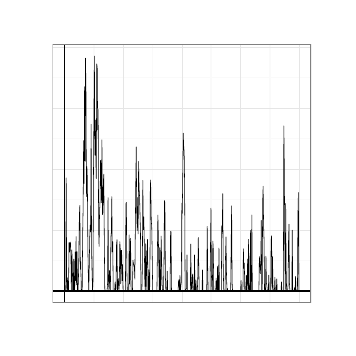
\begin{tikzpicture}[x=1pt,y=1pt]
\definecolor{fillColor}{RGB}{255,255,255}
\path[use as bounding box,fill=fillColor,fill opacity=0.00] (0,0) rectangle (108.41,108.41);
\begin{scope}
\path[clip] (  0.00,  0.00) rectangle (108.40,108.41);
\definecolor{drawColor}{RGB}{255,255,255}
\definecolor{fillColor}{RGB}{255,255,255}

\path[draw=drawColor,line width= 0.6pt,line join=round,line cap=round,fill=fillColor] (  0.00,  0.00) rectangle (108.41,108.41);
\end{scope}
\begin{scope}
\path[clip] (  9.00,  9.00) rectangle (102.41,102.41);
\definecolor{fillColor}{RGB}{255,255,255}

\path[fill=fillColor] (  9.00,  9.00) rectangle (102.40,102.41);
\definecolor{drawColor}{gray}{0.98}

\path[draw=drawColor,line width= 0.6pt,line join=round] (  9.00, 24.26) --
	(102.41, 24.26);

\path[draw=drawColor,line width= 0.6pt,line join=round] (  9.00, 46.29) --
	(102.41, 46.29);

\path[draw=drawColor,line width= 0.6pt,line join=round] (  9.00, 68.33) --
	(102.41, 68.33);

\path[draw=drawColor,line width= 0.6pt,line join=round] (  9.00, 90.36) --
	(102.41, 90.36);

\path[draw=drawColor,line width= 0.6pt,line join=round] ( 23.86,  9.00) --
	( 23.86,102.41);

\path[draw=drawColor,line width= 0.6pt,line join=round] ( 45.09,  9.00) --
	( 45.09,102.41);

\path[draw=drawColor,line width= 0.6pt,line join=round] ( 66.32,  9.00) --
	( 66.32,102.41);

\path[draw=drawColor,line width= 0.6pt,line join=round] ( 87.55,  9.00) --
	( 87.55,102.41);
\definecolor{drawColor}{gray}{0.90}

\path[draw=drawColor,line width= 0.2pt,line join=round] (  9.00, 13.25) --
	(102.41, 13.25);

\path[draw=drawColor,line width= 0.2pt,line join=round] (  9.00, 35.28) --
	(102.41, 35.28);

\path[draw=drawColor,line width= 0.2pt,line join=round] (  9.00, 57.31) --
	(102.41, 57.31);

\path[draw=drawColor,line width= 0.2pt,line join=round] (  9.00, 79.34) --
	(102.41, 79.34);

\path[draw=drawColor,line width= 0.2pt,line join=round] (  9.00,101.37) --
	(102.41,101.37);

\path[draw=drawColor,line width= 0.2pt,line join=round] ( 13.25,  9.00) --
	( 13.25,102.41);

\path[draw=drawColor,line width= 0.2pt,line join=round] ( 34.47,  9.00) --
	( 34.47,102.41);

\path[draw=drawColor,line width= 0.2pt,line join=round] ( 55.70,  9.00) --
	( 55.70,102.41);

\path[draw=drawColor,line width= 0.2pt,line join=round] ( 76.93,  9.00) --
	( 76.93,102.41);

\path[draw=drawColor,line width= 0.2pt,line join=round] ( 98.16,  9.00) --
	( 98.16,102.41);
\definecolor{drawColor}{RGB}{0,0,0}

\path[draw=drawColor,line width= 0.2pt,line join=round] ( 13.25, 13.25) --
	( 13.42, 13.25) --
	( 13.59, 13.25) --
	( 13.76, 13.25) --
	( 13.92, 54.14) --
	( 14.09, 17.38) --
	( 14.26, 13.25) --
	( 14.43, 18.06) --
	( 14.60, 13.25) --
	( 14.77, 13.25) --
	( 14.94, 30.76) --
	( 15.11, 27.29) --
	( 15.28, 30.83) --
	( 15.45, 30.92) --
	( 15.62, 26.45) --
	( 15.79, 13.25) --
	( 15.96, 28.15) --
	( 16.13, 22.92) --
	( 16.30, 13.25) --
	( 16.47, 13.25) --
	( 16.64, 24.80) --
	( 16.81, 13.25) --
	( 16.98, 13.25) --
	( 17.15, 27.35) --
	( 17.32, 17.01) --
	( 17.49, 32.94) --
	( 17.66, 15.46) --
	( 17.83, 27.45) --
	( 18.00, 13.25) --
	( 18.17, 13.25) --
	( 18.34, 17.35) --
	( 18.51, 27.79) --
	( 18.68, 40.67) --
	( 18.85, 44.23) --
	( 19.02, 21.12) --
	( 19.19, 23.88) --
	( 19.36, 13.25) --
	( 19.53, 13.25) --
	( 19.70, 13.25) --
	( 19.87, 33.88) --
	( 20.04, 43.60) --
	( 20.21, 67.62) --
	( 20.38, 52.11) --
	( 20.55, 87.08) --
	( 20.72, 60.24) --
	( 20.89, 97.37) --
	( 21.06, 86.61) --
	( 21.23, 47.36) --
	( 21.40, 58.18) --
	( 21.57, 53.76) --
	( 21.74, 29.57) --
	( 21.91, 19.08) --
	( 22.08, 13.25) --
	( 22.25, 21.89) --
	( 22.42, 32.62) --
	( 22.59, 37.03) --
	( 22.76, 34.61) --
	( 22.93, 73.52) --
	( 23.10, 27.83) --
	( 23.27, 19.90) --
	( 23.44, 13.25) --
	( 23.61, 16.74) --
	( 23.77, 54.45) --
	( 23.94, 78.67) --
	( 24.11, 98.16) --
	( 24.28, 62.36) --
	( 24.45, 75.06) --
	( 24.62, 61.26) --
	( 24.79, 53.88) --
	( 24.96, 95.31) --
	( 25.13, 93.93) --
	( 25.30, 71.48) --
	( 25.47, 78.86) --
	( 25.64, 35.31) --
	( 25.81, 29.37) --
	( 25.98, 42.04) --
	( 26.15, 45.55) --
	( 26.32, 60.48) --
	( 26.49, 58.43) --
	( 26.66, 45.15) --
	( 26.83, 67.90) --
	( 27.00, 40.84) --
	( 27.17, 41.65) --
	( 27.34, 52.71) --
	( 27.51, 55.49) --
	( 27.68, 33.32) --
	( 27.85, 14.15) --
	( 28.02, 13.25) --
	( 28.19, 13.25) --
	( 28.36, 13.25) --
	( 28.53, 13.25) --
	( 28.70, 13.25) --
	( 28.87, 16.06) --
	( 29.04, 46.96) --
	( 29.21, 16.72) --
	( 29.38, 13.25) --
	( 29.55, 20.68) --
	( 29.72, 16.83) --
	( 29.89, 13.25) --
	( 30.06, 32.57) --
	( 30.23, 34.48) --
	( 30.40, 47.35) --
	( 30.57, 27.36) --
	( 30.74, 31.06) --
	( 30.91, 13.25) --
	( 31.08, 13.25) --
	( 31.25, 13.25) --
	( 31.42, 13.25) --
	( 31.59, 16.53) --
	( 31.76, 13.25) --
	( 31.93, 14.18) --
	( 32.10, 29.93) --
	( 32.27, 31.79) --
	( 32.44, 13.25) --
	( 32.61, 16.58) --
	( 32.78, 17.72) --
	( 32.95, 13.25) --
	( 33.12, 15.66) --
	( 33.29, 31.08) --
	( 33.46, 28.50) --
	( 33.62, 15.82) --
	( 33.79, 27.92) --
	( 33.96, 27.93) --
	( 34.13, 17.00) --
	( 34.30, 22.82) --
	( 34.47, 13.25) --
	( 34.64, 13.25) --
	( 34.81, 13.25) --
	( 34.98, 13.25) --
	( 35.15, 13.25) --
	( 35.32, 13.25) --
	( 35.49, 44.72) --
	( 35.66, 45.31) --
	( 35.83, 22.31) --
	( 36.00, 13.25) --
	( 36.17, 13.25) --
	( 36.34, 13.25) --
	( 36.51, 13.25) --
	( 36.68, 33.52) --
	( 36.85, 15.77) --
	( 37.02, 25.43) --
	( 37.19, 32.32) --
	( 37.36, 13.25) --
	( 37.53, 13.25) --
	( 37.70, 13.25) --
	( 37.87, 13.25) --
	( 38.04, 24.39) --
	( 38.21, 23.14) --
	( 38.38, 22.69) --
	( 38.55, 21.83) --
	( 38.72, 17.54) --
	( 38.89, 34.77) --
	( 39.06, 52.67) --
	( 39.23, 65.30) --
	( 39.40, 42.27) --
	( 39.57, 35.11) --
	( 39.74, 47.05) --
	( 39.91, 33.87) --
	( 40.08, 60.09) --
	( 40.25, 50.58) --
	( 40.42, 47.55) --
	( 40.59, 41.22) --
	( 40.76, 34.22) --
	( 40.93, 13.25) --
	( 41.10, 13.25) --
	( 41.27, 13.25) --
	( 41.44, 21.71) --
	( 41.61, 53.22) --
	( 41.78, 35.41) --
	( 41.95, 40.03) --
	( 42.12, 31.83) --
	( 42.29, 18.14) --
	( 42.46, 13.25) --
	( 42.63, 30.33) --
	( 42.80, 13.25) --
	( 42.97, 20.57) --
	( 43.14, 28.66) --
	( 43.31, 31.91) --
	( 43.47, 13.25) --
	( 43.64, 13.25) --
	( 43.81, 20.93) --
	( 43.98, 13.25) --
	( 44.15, 15.33) --
	( 44.32, 53.37) --
	( 44.49, 50.33) --
	( 44.66, 38.95) --
	( 44.83, 36.19) --
	( 45.00, 26.28) --
	( 45.17, 13.25) --
	( 45.34, 13.25) --
	( 45.51, 13.25) --
	( 45.68, 13.25) --
	( 45.85, 13.25) --
	( 46.02, 13.25) --
	( 46.19, 13.25) --
	( 46.36, 13.25) --
	( 46.53, 13.25) --
	( 46.70, 13.25) --
	( 46.87, 26.90) --
	( 47.04, 40.70) --
	( 47.21, 33.58) --
	( 47.38, 22.85) --
	( 47.55, 13.25) --
	( 47.72, 28.92) --
	( 47.89, 13.25) --
	( 48.06, 13.25) --
	( 48.23, 33.12) --
	( 48.40, 25.02) --
	( 48.57, 16.20) --
	( 48.74, 13.25) --
	( 48.91, 13.25) --
	( 49.08, 13.25) --
	( 49.25, 22.65) --
	( 49.42, 45.93) --
	( 49.59, 45.06) --
	( 49.76, 18.80) --
	( 49.93, 13.25) --
	( 50.10, 13.25) --
	( 50.27, 13.25) --
	( 50.44, 20.39) --
	( 50.61, 13.25) --
	( 50.78, 13.25) --
	( 50.95, 13.25) --
	( 51.12, 13.25) --
	( 51.29, 13.25) --
	( 51.46, 13.25) --
	( 51.63, 34.82) --
	( 51.80, 34.71) --
	( 51.97, 13.25) --
	( 52.14, 13.25) --
	( 52.31, 13.25) --
	( 52.48, 13.25) --
	( 52.65, 13.25) --
	( 52.82, 13.25) --
	( 52.99, 13.25) --
	( 53.16, 13.25) --
	( 53.32, 13.25) --
	( 53.49, 13.25) --
	( 53.66, 13.25) --
	( 53.83, 13.25) --
	( 54.00, 13.25) --
	( 54.17, 13.25) --
	( 54.34, 13.25) --
	( 54.51, 16.72) --
	( 54.68, 17.33) --
	( 54.85, 13.25) --
	( 55.02, 18.87) --
	( 55.19, 13.25) --
	( 55.36, 15.23) --
	( 55.53, 16.49) --
	( 55.70, 45.04) --
	( 55.87, 41.32) --
	( 56.04, 55.44) --
	( 56.21, 70.28) --
	( 56.38, 65.61) --
	( 56.55, 63.33) --
	( 56.72, 51.37) --
	( 56.89, 13.25) --
	( 57.06, 13.25) --
	( 57.23, 13.88) --
	( 57.40, 14.31) --
	( 57.57, 26.29) --
	( 57.74, 13.25) --
	( 57.91, 13.25) --
	( 58.08, 13.25) --
	( 58.25, 13.25) --
	( 58.42, 13.25) --
	( 58.59, 13.25) --
	( 58.76, 13.25) --
	( 58.93, 30.23) --
	( 59.10, 15.42) --
	( 59.27, 13.25) --
	( 59.44, 17.93) --
	( 59.61, 19.42) --
	( 59.78, 13.25) --
	( 59.95, 13.25) --
	( 60.12, 13.25) --
	( 60.29, 26.30) --
	( 60.46, 13.25) --
	( 60.63, 13.25) --
	( 60.80, 17.23) --
	( 60.97, 13.25) --
	( 61.14, 13.25) --
	( 61.31, 13.25) --
	( 61.48, 18.60) --
	( 61.65, 32.58) --
	( 61.82, 22.76) --
	( 61.99, 13.25) --
	( 62.16, 13.25) --
	( 62.33, 13.25) --
	( 62.50, 13.25) --
	( 62.67, 13.25) --
	( 62.84, 13.25) --
	( 63.01, 13.25) --
	( 63.17, 20.92) --
	( 63.34, 13.25) --
	( 63.51, 13.25) --
	( 63.68, 13.25) --
	( 63.85, 13.25) --
	( 64.02, 13.25) --
	( 64.19, 13.25) --
	( 64.36, 13.25) --
	( 64.53, 13.25) --
	( 64.70, 13.25) --
	( 64.87, 36.61) --
	( 65.04, 22.65) --
	( 65.21, 13.25) --
	( 65.38, 13.25) --
	( 65.55, 13.25) --
	( 65.72, 13.25) --
	( 65.89, 13.25) --
	( 66.06, 29.79) --
	( 66.23, 43.18) --
	( 66.40, 19.25) --
	( 66.57, 13.25) --
	( 66.74, 13.25) --
	( 66.91, 31.27) --
	( 67.08, 28.14) --
	( 67.25, 13.25) --
	( 67.42, 13.25) --
	( 67.59, 13.25) --
	( 67.76, 13.25) --
	( 67.93, 13.25) --
	( 68.10, 17.91) --
	( 68.27, 13.25) --
	( 68.44, 13.25) --
	( 68.61, 22.21) --
	( 68.78, 13.25) --
	( 68.95, 13.25) --
	( 69.12, 28.78) --
	( 69.29, 13.25) --
	( 69.46, 13.25) --
	( 69.63, 13.25) --
	( 69.80, 13.25) --
	( 69.97, 13.25) --
	( 70.14, 36.88) --
	( 70.31, 34.72) --
	( 70.48, 48.44) --
	( 70.65, 23.53) --
	( 70.82, 14.08) --
	( 70.99, 13.25) --
	( 71.16, 13.25) --
	( 71.33, 13.25) --
	( 71.50, 26.43) --
	( 71.67, 32.79) --
	( 71.84, 19.45) --
	( 72.01, 13.25) --
	( 72.18, 14.20) --
	( 72.35, 13.25) --
	( 72.52, 13.25) --
	( 72.69, 13.25) --
	( 72.86, 13.25) --
	( 73.02, 13.25) --
	( 73.19, 13.25) --
	( 73.36, 13.25) --
	( 73.53, 30.53) --
	( 73.70, 44.01) --
	( 73.87, 16.59) --
	( 74.04, 13.25) --
	( 74.21, 13.25) --
	( 74.38, 13.25) --
	( 74.55, 13.25) --
	( 74.72, 13.25) --
	( 74.89, 13.25) --
	( 75.06, 13.25) --
	( 75.23, 13.25) --
	( 75.40, 13.25) --
	( 75.57, 13.25) --
	( 75.74, 13.25) --
	( 75.91, 13.25) --
	( 76.08, 13.25) --
	( 76.25, 13.25) --
	( 76.42, 13.25) --
	( 76.59, 13.25) --
	( 76.76, 13.25) --
	( 76.93, 13.25) --
	( 77.10, 17.10) --
	( 77.27, 13.25) --
	( 77.44, 13.25) --
	( 77.61, 13.25) --
	( 77.78, 13.25) --
	( 77.95, 28.53) --
	( 78.12, 21.40) --
	( 78.29, 23.31) --
	( 78.46, 13.25) --
	( 78.63, 13.25) --
	( 78.80, 13.25) --
	( 78.97, 18.87) --
	( 79.14, 13.25) --
	( 79.31, 17.28) --
	( 79.48, 24.85) --
	( 79.65, 13.25) --
	( 79.82, 31.93) --
	( 79.99, 13.25) --
	( 80.16, 13.25) --
	( 80.33, 13.25) --
	( 80.50, 35.18) --
	( 80.67, 13.25) --
	( 80.84, 13.25) --
	( 81.01, 40.73) --
	( 81.18, 13.25) --
	( 81.35, 13.25) --
	( 81.52, 13.25) --
	( 81.69, 13.25) --
	( 81.86, 13.25) --
	( 82.03, 13.25) --
	( 82.20, 13.25) --
	( 82.37, 13.25) --
	( 82.54, 13.25) --
	( 82.71, 13.25) --
	( 82.87, 13.25) --
	( 83.04, 13.25) --
	( 83.21, 13.25) --
	( 83.38, 13.25) --
	( 83.55, 13.25) --
	( 83.72, 25.69) --
	( 83.89, 23.53) --
	( 84.06, 19.51) --
	( 84.23, 22.87) --
	( 84.40, 38.73) --
	( 84.57, 13.25) --
	( 84.74, 13.25) --
	( 84.91, 45.47) --
	( 85.08, 51.12) --
	( 85.25, 36.99) --
	( 85.42, 31.74) --
	( 85.59, 13.25) --
	( 85.76, 13.25) --
	( 85.93, 13.25) --
	( 86.10, 25.81) --
	( 86.27, 16.17) --
	( 86.44, 15.10) --
	( 86.61, 13.25) --
	( 86.78, 13.25) --
	( 86.95, 13.25) --
	( 87.12, 18.96) --
	( 87.29, 13.25) --
	( 87.46, 13.25) --
	( 87.63, 13.25) --
	( 87.80, 13.25) --
	( 87.97, 31.67) --
	( 88.14, 33.24) --
	( 88.31, 13.25) --
	( 88.48, 25.69) --
	( 88.65, 14.55) --
	( 88.82, 13.25) --
	( 88.99, 13.25) --
	( 89.16, 13.25) --
	( 89.33, 18.25) --
	( 89.50, 13.25) --
	( 89.67, 13.25) --
	( 89.84, 13.25) --
	( 90.01, 17.65) --
	( 90.18, 13.25) --
	( 90.35, 13.25) --
	( 90.52, 13.25) --
	( 90.69, 13.25) --
	( 90.86, 13.25) --
	( 91.03, 13.25) --
	( 91.20, 13.25) --
	( 91.37, 13.25) --
	( 91.54, 13.25) --
	( 91.71, 16.57) --
	( 91.88, 13.25) --
	( 92.05, 13.25) --
	( 92.22, 13.25) --
	( 92.39, 13.25) --
	( 92.56, 72.91) --
	( 92.72, 59.64) --
	( 92.89, 31.42) --
	( 93.06, 13.25) --
	( 93.23, 44.88) --
	( 93.40, 21.58) --
	( 93.57, 13.25) --
	( 93.74, 13.25) --
	( 93.91, 13.25) --
	( 94.08, 15.22) --
	( 94.25, 31.27) --
	( 94.42, 37.43) --
	( 94.59, 16.05) --
	( 94.76, 13.25) --
	( 94.93, 13.25) --
	( 95.10, 13.25) --
	( 95.27, 13.25) --
	( 95.44, 13.25) --
	( 95.61, 35.25) --
	( 95.78, 13.25) --
	( 95.95, 13.25) --
	( 96.12, 13.25) --
	( 96.29, 13.25) --
	( 96.46, 14.53) --
	( 96.63, 13.25) --
	( 96.80, 18.56) --
	( 96.97, 13.25) --
	( 97.14, 13.25) --
	( 97.31, 13.25) --
	( 97.48, 13.25) --
	( 97.65, 40.55) --
	( 97.82, 48.86) --
	( 97.99, 13.25) --
	( 98.16, 13.25);

\path[draw=drawColor,line width= 0.6pt,line join=round] (  9.00, 13.25) -- (102.41, 13.25);

\path[draw=drawColor,line width= 0.6pt,line join=round] ( 13.25,  9.00) -- ( 13.25,102.41);
\definecolor{drawColor}{gray}{0.50}

\path[draw=drawColor,line width= 0.6pt,line join=round,line cap=round] (  9.00,  9.00) rectangle (102.40,102.41);
\end{scope}
\end{tikzpicture}
}%
	\caption{A sample Brownian motion, Brownian motion with drift and with reflection for $\pp_1>0$ and $\pp_2<0$.}%
	\label{F: BM}%
\end{figure}

See Figure~\ref{F: BM} for an example of a Brownian motion with drift for positive and negative $\pp$ and the corresponding reflected process.
Note that for positive $t$ the time intervals between zeroes of $\Bt$ are much longer than for negative $\pp$.
We call an excursion $\gamma$ of $\Bt$ a time interval $[l(\gamma), r(\gamma)]$ for which $\Bt(l(\gamma)) = \Bt(r(\gamma)) = 0$
and $\Bt(s) > 0$ for all $l(\gamma) < s < r(\gamma)$.
Denote by $|\gamma| = r(\gamma) - l(\gamma)$ the length of an excursion.

Additionally we define a Poisson counting process $\Nt$, 
which equips each excursion with a number of marks,
emerging with intensity $\Bt(s)$ at time $s$.
Informally speaking, the chance of encountering a mark in a time interval $\sds$ is characterized by
\begin{equation}
	\Prob( \text{Some mark emerges in} \; \sds \cond \Bt(u), u \leq s ) = \Bt(s)ds.
\end{equation}
More formally we define $\Nt$ to be the counting process for which
\begin{equation}
	\Nt(s) - \int_{0}^{s} \Bt(s)ds
\end{equation}
is a martingale.
Denote by $\mu(\gamma)$ the number of marks during an excursion $\gamma$.

We now state the main theorem of this thesis, which we will prove gradually in the following chapters.
\begin{theorem}[Main theorem] \label{T: Main}
	Let 
	$\Cnt(1) \geq \Cnt(2) \geq ... $ 
	be the ordered component sizes of 
	$\Gnt$
	and let
	$\sigmant(j)$ 
	be the surplus of the corresponding component.
	Then, as $n \rightarrow \infty$,
	\begin{equation}
	( \n{-2}{3} ( \Cnt(j), \sigmant(j) ), \; j \geq 1 ) 
	\rightarrow_d
	( (\Ct(j), \sigmat), \; j \geq 1 )
	= ( \Ctbold, \sigmatbold ),
	\end{equation}
	where the convergence 
	$\n{-2}{3} \Cntbold \rightarrow_p \Ctbold$
	holds with respect to the $\ld$ topology.
	
	The limit
	$\left( ( \Ct(j), \sigmat(j) ), \; j \geq 1 \right)$
	is distributed as the sequence
	$ \left( (|\gamma_j|, \mu(\gamma_j)), j \geq 1  \right) $
	of lengths and mark-counts of excursions of $\Bt$.
\end{theorem}
\fxfatal{ld topology must be explained or removed.}

We conclude this chapter with an overview of the remaining chapters and the structure of the proof of Theorem~\ref{T: Main}.

Chapter~\ref{C: preliminaries} will develop some preliminary theory on the function spaces $C$ and $D$,
convergence of probability measures and counting processes, which will prove useful in the coming chapters.

In Chapter~\ref{C: bf-walk} we define a way to traverse all vertices of a given graph, called the breadth-first walk $\znt$, 
that reduces the graph to a one-dimensional random walk in which component sizes are decoded as excursions above past minima.
We analyse its characteristics when applied to $\Gnt$ and discover that, after a certain rescaling, it converges in distribution to $\Wt$.

Chapter~\ref{C: surplus edges} deals with the second coordinate $\sigmant$ in Theorem~\ref{T: Main}, the surplus edges.
We describe a Poisson counting process $\nnt$ which tallies up all encountered excess edges and calculate its limit rate as $\Bt$.
The remainder of this chapter will be spent proving that this convergence of rates suffices to declare the convergence of the joint distribution of
the rescaled breadth-first walk and this counting process to $\Wt$ and $\Nt$.

It remains to be proven that not only does the rescaled random walk converge in distribution to the Brownian motion with drift,
but that the convergence of component sizes to lengths of excursions of $\Bt$ in distribution follows as well.
In Chapter~\ref{C: convergence} we first prove that this does indeed hold if we must not expect any large components to "wander off to infinity" as $n \rightarrow \infty$ and subsequently that, with high probability, this problem does not arise in $\Gnt$.
This completes the proof of Theorem~\ref{T: Main}.

Lastly, Chapter~\ref{C: outlook} provides an overview over the remaining statements of Aldous paper,
which contains a non-uniform version of Theorem~\ref{T: Main} and the multiplicative coalescent, 
a process describing the joining of components to form larger components as the parameter $\pp$ grows.

